\documentclass{scrreprt}\usepackage[]{graphicx}\usepackage[]{color}
%% maxwidth is the original width if it is less than linewidth
%% otherwise use linewidth (to make sure the graphics do not exceed the margin)
\makeatletter
\def\maxwidth{ %
  \ifdim\Gin@nat@width>\linewidth
    \linewidth
  \else
    \Gin@nat@width
  \fi
}
\makeatother

\definecolor{fgcolor}{rgb}{0.345, 0.345, 0.345}
\newcommand{\hlnum}[1]{\textcolor[rgb]{0.686,0.059,0.569}{#1}}%
\newcommand{\hlstr}[1]{\textcolor[rgb]{0.192,0.494,0.8}{#1}}%
\newcommand{\hlcom}[1]{\textcolor[rgb]{0.678,0.584,0.686}{\textit{#1}}}%
\newcommand{\hlopt}[1]{\textcolor[rgb]{0,0,0}{#1}}%
\newcommand{\hlstd}[1]{\textcolor[rgb]{0.345,0.345,0.345}{#1}}%
\newcommand{\hlkwa}[1]{\textcolor[rgb]{0.161,0.373,0.58}{\textbf{#1}}}%
\newcommand{\hlkwb}[1]{\textcolor[rgb]{0.69,0.353,0.396}{#1}}%
\newcommand{\hlkwc}[1]{\textcolor[rgb]{0.333,0.667,0.333}{#1}}%
\newcommand{\hlkwd}[1]{\textcolor[rgb]{0.737,0.353,0.396}{\textbf{#1}}}%

\usepackage{framed}
\makeatletter
\newenvironment{kframe}{%
 \def\at@end@of@kframe{}%
 \ifinner\ifhmode%
  \def\at@end@of@kframe{\end{minipage}}%
  \begin{minipage}{\columnwidth}%
 \fi\fi%
 \def\FrameCommand##1{\hskip\@totalleftmargin \hskip-\fboxsep
 \colorbox{shadecolor}{##1}\hskip-\fboxsep
     % There is no \\@totalrightmargin, so:
     \hskip-\linewidth \hskip-\@totalleftmargin \hskip\columnwidth}%
 \MakeFramed {\advance\hsize-\width
   \@totalleftmargin\z@ \linewidth\hsize
   \@setminipage}}%
 {\par\unskip\endMakeFramed%
 \at@end@of@kframe}
\makeatother

\definecolor{shadecolor}{rgb}{.97, .97, .97}
\definecolor{messagecolor}{rgb}{0, 0, 0}
\definecolor{warningcolor}{rgb}{1, 0, 1}
\definecolor{errorcolor}{rgb}{1, 0, 0}
\newenvironment{knitrout}{}{} % an empty environment to be redefined in TeX

\usepackage{alltt}
\usepackage[landscape,twocolumn]{geometry}
\newlength\figurewidth
\setlength\figurewidth\columnwidth
\title{Flights 1987-2015}
\author{Hugh P}
\IfFileExists{upquote.sty}{\usepackage{upquote}}{}
\begin{document}
\begin{knitrout}
\definecolor{shadecolor}{rgb}{0.969, 0.969, 0.969}\color{fgcolor}\begin{kframe}
\begin{alltt}
\hlstd{START.TIME} \hlkwb{<-} \hlkwd{Sys.time}\hlstd{()}
\hlstd{knitr}\hlopt{::}\hlstd{opts_chunk}\hlopt{$}\hlkwd{set}\hlstd{(}\hlkwc{fig.show} \hlstd{=} \hlstr{'hide'}\hlstd{,}
                      \hlkwc{fig.width} \hlstd{=} \hlnum{11}\hlstd{,}
                      \hlkwc{fig.height} \hlstd{=} \hlnum{7}\hlstd{,}
                      \hlkwc{out.width} \hlstd{=} \hlstr{"11in"}\hlstd{)}
\end{alltt}
\end{kframe}
\end{knitrout}

\begin{knitrout}
\definecolor{shadecolor}{rgb}{0.969, 0.969, 0.969}\color{fgcolor}\begin{kframe}
\begin{alltt}
\hlkwd{library}\hlstd{(data.table)}
\hlkwd{library}\hlstd{(bit64)}
\end{alltt}


{\ttfamily\noindent\itshape\color{messagecolor}{\#\# Loading required package: bit\\\#\# Attaching package bit\\\#\# package:bit (c) 2008-2012 Jens Oehlschlaegel (GPL-2)\\\#\# creators: bit bitwhich\\\#\# coercion: as.logical as.integer as.bit as.bitwhich which\\\#\# operator: ! \& | xor != ==\\\#\# querying: print length any all min max range sum summary\\\#\# bit access: length<- [ [<- [[ [[<-\\\#\# for more help type ?bit\\\#\# \\\#\# Attaching package: 'bit'\\\#\# \\\#\# The following object is masked from 'package:data.table':\\\#\# \\\#\#\ \ \ \  setattr\\\#\# \\\#\# The following object is masked from 'package:base':\\\#\# \\\#\#\ \ \ \  xor\\\#\# \\\#\# Attaching package bit64\\\#\# package:bit64 (c) 2011-2012 Jens Oehlschlaegel (GPL-2 with commercial restrictions)\\\#\# creators: integer64 seq :\\\#\# coercion: as.integer64 as.vector as.logical as.integer as.double as.character as.bin\\\#\# logical operator: ! \& | xor != == < <= >= >\\\#\# arithmetic operator: + - * / \%/\% \%\% \textasciicircum{}\\\#\# math: sign abs sqrt log log2 log10\\\#\# math: floor ceiling trunc round\\\#\# querying: is.integer64 is.vector [is.atomic\} [length] is.na format print\\\#\# aggregation: any all min max range sum prod\\\#\# cumulation: diff cummin cummax cumsum cumprod\\\#\# access: length<- [ [<- [[ [[<-\\\#\# combine: c rep cbind rbind as.data.frame\\\#\# for more help type ?bit64\\\#\# \\\#\# Attaching package: 'bit64'\\\#\# \\\#\# The following object is masked from 'package:bit':\\\#\# \\\#\#\ \ \ \  still.identical\\\#\# \\\#\# The following objects are masked from 'package:base':\\\#\# \\\#\#\ \ \ \  \%in\%, :, is.double, match, order, rank}}\begin{alltt}
\hlkwd{library}\hlstd{(dplyr)}
\end{alltt}


{\ttfamily\noindent\itshape\color{messagecolor}{\#\# \\\#\# Attaching package: 'dplyr'\\\#\# \\\#\# The following objects are masked from 'package:data.table':\\\#\# \\\#\#\ \ \ \  between, last\\\#\# \\\#\# The following objects are masked from 'package:stats':\\\#\# \\\#\#\ \ \ \  filter, lag\\\#\# \\\#\# The following objects are masked from 'package:base':\\\#\# \\\#\#\ \ \ \  intersect, setdiff, setequal, union}}\begin{alltt}
\hlkwd{library}\hlstd{(magrittr)}
\hlkwd{library}\hlstd{(ggplot2)}
\hlkwd{theme_update}\hlstd{(}\hlkwc{text} \hlstd{=} \hlkwd{element_text}\hlstd{(}\hlkwc{family} \hlstd{=} \hlstr{""}\hlstd{,}
                                 \hlkwc{face} \hlstd{=} \hlstr{"plain"}\hlstd{,} \hlkwc{colour} \hlstd{=} \hlstr{"black"}\hlstd{,} \hlkwc{size} \hlstd{=} \hlnum{20}\hlstd{,} \hlkwc{lineheight} \hlstd{=} \hlnum{0.9}\hlstd{,}
                                 \hlkwc{hjust} \hlstd{=} \hlnum{0.5}\hlstd{,} \hlkwc{vjust} \hlstd{=} \hlnum{0.5}\hlstd{,} \hlkwc{angle} \hlstd{=} \hlnum{0}\hlstd{,} \hlkwc{margin} \hlstd{=} \hlkwd{margin}\hlstd{(),}
                                 \hlkwc{debug} \hlstd{=} \hlnum{FALSE}\hlstd{))}
\hlkwd{library}\hlstd{(nycflights13)}  \hlcom{# for airports}
\hlstd{nycflights.airports} \hlkwb{<-} \hlstd{airports}
\hlkwd{library}\hlstd{(fasttime)}
\hlkwd{library}\hlstd{(grattan)}
\end{alltt}


{\ttfamily\noindent\itshape\color{messagecolor}{\#\# \\\#\# Attaching package: 'grattan'\\\#\# \\\#\# The following object is masked from 'package:datasets':\\\#\# \\\#\#\ \ \ \  Orange}}\begin{alltt}
\hlkwd{library}\hlstd{(directlabels)}
\end{alltt}
\end{kframe}
\end{knitrout}

\begin{knitrout}
\definecolor{shadecolor}{rgb}{0.969, 0.969, 0.969}\color{fgcolor}\begin{kframe}
\begin{alltt}
\hlstd{pre2008_flights} \hlkwb{<-}
  \hlkwd{rbindlist}\hlstd{(}\hlkwd{lapply}\hlstd{(}\hlkwd{list.files}\hlstd{(}\hlkwc{path} \hlstd{=} \hlstr{"../flights/1987-2008/"}\hlstd{,}
                    \hlkwc{pattern} \hlstd{=} \hlstr{"csv$"}\hlstd{,}
                    \hlkwc{full.names} \hlstd{=} \hlnum{TRUE}\hlstd{), fread))}

\hlstd{pre2008.names} \hlkwb{<-}
  \hlkwd{names}\hlstd{(pre2008_flights)}

\hlstd{read_and_report} \hlkwb{<-}
  \hlkwa{function}\hlstd{(}\hlkwc{filename}\hlstd{)\{}
    \hlstd{year} \hlkwb{<-} \hlkwd{gsub}\hlstd{(}\hlstr{"^.*(2[0-9]\{3\}).\{3,4\}csv$"}\hlstd{,} \hlstr{"\textbackslash{}\textbackslash{}1"}\hlstd{, filename)}
    \hlkwa{if}\hlstd{(}\hlkwd{grepl}\hlstd{(}\hlstr{"1.csv"}\hlstd{, filename,} \hlkwc{fixed} \hlstd{=} \hlnum{TRUE}\hlstd{))}
      \hlkwd{cat}\hlstd{(year)}
    \hlkwd{fread}\hlstd{(filename,} \hlkwc{select} \hlstd{= pre2008.names,} \hlkwc{showProgress} \hlstd{=} \hlnum{FALSE}\hlstd{)}
  \hlstd{\}}

\hlkwd{gc}\hlstd{(}\hlnum{1}\hlstd{,}\hlnum{1}\hlstd{)}
\hlstd{post2008_flights} \hlkwb{<-}
  \hlkwd{rbindlist}\hlstd{(}\hlkwd{lapply}\hlstd{(}\hlkwd{list.files}\hlstd{(}\hlkwc{path} \hlstd{=} \hlstr{"../flights"}\hlstd{,} \hlkwc{recursive} \hlstd{=} \hlnum{TRUE}\hlstd{,} \hlkwc{pattern} \hlstd{=} \hlstr{"2[0-9]\{3\}.\{3,4\}csv$"}\hlstd{,}
                              \hlkwc{full.names} \hlstd{=} \hlnum{TRUE}\hlstd{),}
                   \hlstd{read_and_report))}

\hlstd{flights} \hlkwb{<-} \hlkwd{rbindlist}\hlstd{(}\hlkwd{list}\hlstd{(pre2008_flights, post2008_flights),} \hlkwc{use.names} \hlstd{=} \hlnum{TRUE}\hlstd{)}
\hlstd{readr}\hlopt{::}\hlkwd{write_csv}\hlstd{(flights,} \hlkwc{path} \hlstd{=} \hlstr{"../1987-2015-On-Time-Performance.csv"}\hlstd{)}
\end{alltt}
\end{kframe}
\end{knitrout}

\begin{knitrout}
\definecolor{shadecolor}{rgb}{0.969, 0.969, 0.969}\color{fgcolor}\begin{kframe}
\begin{alltt}
\hlkwd{Sys.time}\hlstd{()}
\end{alltt}
\begin{verbatim}
## [1] "2016-01-12 00:29:32 AEDT"
\end{verbatim}
\begin{alltt}
\hlstd{flights} \hlkwb{<-} \hlkwd{fread}\hlstd{(}\hlstr{"../1987-2015-On-Time-Performance.csv"}\hlstd{,} \hlkwc{select} \hlstd{=} \hlkwd{c}\hlstd{(}\hlstr{"Year"}\hlstd{,} \hlstr{"Month"}\hlstd{,} \hlstr{"DayofMonth"}\hlstd{,} \hlstr{"DepTime"}\hlstd{,} \hlstr{"ArrTime"}\hlstd{,} \hlstr{"UniqueCarrier"}\hlstd{,}
                                                                    \hlstr{"ActualElapsedTime"}\hlstd{,} \hlstr{"ArrDelay"}\hlstd{,} \hlstr{"DepDelay"}\hlstd{,} \hlstr{"Origin"}\hlstd{,} \hlstr{"Dest"}\hlstd{,} \hlstr{"Cancelled"}\hlstd{))}
\end{alltt}
\begin{verbatim}
## 
Read 0.0% of 165931626 rows
Read 0.8% of 165931626 rows
Read 1.6% of 165931626 rows
Read 2.4% of 165931626 rows
Read 3.2% of 165931626 rows
Read 4.0% of 165931626 rows
Read 4.8% of 165931626 rows
Read 5.7% of 165931626 rows
Read 6.5% of 165931626 rows
Read 7.3% of 165931626 rows
Read 8.1% of 165931626 rows
Read 9.0% of 165931626 rows
Read 9.8% of 165931626 rows
Read 10.6% of 165931626 rows
Read 11.5% of 165931626 rows
Read 12.3% of 165931626 rows
Read 13.1% of 165931626 rows
Read 14.0% of 165931626 rows
Read 14.8% of 165931626 rows
Read 15.6% of 165931626 rows
Read 16.5% of 165931626 rows
Read 17.3% of 165931626 rows
Read 18.1% of 165931626 rows
Read 19.0% of 165931626 rows
Read 19.8% of 165931626 rows
Read 20.6% of 165931626 rows
Read 21.5% of 165931626 rows
Read 22.3% of 165931626 rows
Read 23.1% of 165931626 rows
Read 23.9% of 165931626 rows
Read 24.8% of 165931626 rows
Read 25.6% of 165931626 rows
Read 26.4% of 165931626 rows
Read 27.2% of 165931626 rows
Read 28.1% of 165931626 rows
Read 28.9% of 165931626 rows
Read 29.7% of 165931626 rows
Read 30.5% of 165931626 rows
Read 31.4% of 165931626 rows
Read 32.2% of 165931626 rows
Read 33.0% of 165931626 rows
Read 33.8% of 165931626 rows
Read 34.7% of 165931626 rows
Read 35.5% of 165931626 rows
Read 36.3% of 165931626 rows
Read 37.1% of 165931626 rows
Read 38.0% of 165931626 rows
Read 38.8% of 165931626 rows
Read 39.6% of 165931626 rows
Read 40.4% of 165931626 rows
Read 41.3% of 165931626 rows
Read 42.1% of 165931626 rows
Read 42.9% of 165931626 rows
Read 43.7% of 165931626 rows
Read 44.6% of 165931626 rows
Read 45.4% of 165931626 rows
Read 46.2% of 165931626 rows
Read 47.0% of 165931626 rows
Read 47.8% of 165931626 rows
Read 48.7% of 165931626 rows
Read 49.5% of 165931626 rows
Read 50.3% of 165931626 rows
Read 51.1% of 165931626 rows
Read 52.0% of 165931626 rows
Read 52.8% of 165931626 rows
Read 53.6% of 165931626 rows
Read 54.4% of 165931626 rows
Read 55.3% of 165931626 rows
Read 56.1% of 165931626 rows
Read 56.9% of 165931626 rows
Read 57.7% of 165931626 rows
Read 58.5% of 165931626 rows
Read 59.3% of 165931626 rows
Read 60.2% of 165931626 rows
Read 61.0% of 165931626 rows
Read 61.8% of 165931626 rows
Read 62.6% of 165931626 rows
Read 63.4% of 165931626 rows
Read 64.3% of 165931626 rows
Read 65.1% of 165931626 rows
Read 65.9% of 165931626 rows
Read 66.7% of 165931626 rows
Read 67.5% of 165931626 rows
Read 68.4% of 165931626 rows
Read 69.2% of 165931626 rows
Read 70.0% of 165931626 rows
Read 70.8% of 165931626 rows
Read 71.6% of 165931626 rows
Read 72.4% of 165931626 rows
Read 73.2% of 165931626 rows
Read 74.0% of 165931626 rows
Read 74.9% of 165931626 rows
Read 75.7% of 165931626 rows
Read 76.5% of 165931626 rows
Read 77.3% of 165931626 rows
Read 78.1% of 165931626 rows
Read 78.9% of 165931626 rows
Read 79.7% of 165931626 rows
Read 80.6% of 165931626 rows
Read 81.4% of 165931626 rows
Read 82.2% of 165931626 rows
Read 83.0% of 165931626 rows
Read 83.8% of 165931626 rows
Read 84.6% of 165931626 rows
Read 85.4% of 165931626 rows
Read 86.3% of 165931626 rows
Read 87.1% of 165931626 rows
Read 87.9% of 165931626 rows
Read 88.7% of 165931626 rows
Read 89.5% of 165931626 rows
Read 90.3% of 165931626 rows
Read 91.1% of 165931626 rows
Read 91.9% of 165931626 rows
Read 92.8% of 165931626 rows
Read 93.6% of 165931626 rows
Read 94.4% of 165931626 rows
Read 95.2% of 165931626 rows
Read 96.0% of 165931626 rows
Read 96.8% of 165931626 rows
Read 97.6% of 165931626 rows
Read 98.4% of 165931626 rows
Read 99.2% of 165931626 rows
Read 165931626 rows and 12 (of 29) columns from 15.111 GB file in 00:02:25
\end{verbatim}
\begin{alltt}
\hlcom{# flights <- readRDS("../1987-2015-On-Time-Performance.rds")}
\end{alltt}
\end{kframe}
\end{knitrout}

\begin{knitrout}
\definecolor{shadecolor}{rgb}{0.969, 0.969, 0.969}\color{fgcolor}\begin{kframe}
\begin{alltt}
\hlstd{flightsSanFran} \hlkwb{<-} \hlstd{flights[Origin} \hlopt \hlkwd{c}\hlstd{(}\hlstr{"SFO"}\hlstd{,} \hlstr{"OAK"}\hlstd{)} \hlopt{|} \hlstd{Dest} \hlopt \hlkwd{c}\hlstd{(}\hlstr{"SFO"}\hlstd{,} \hlstr{"OAK"}\hlstd{)]}
\hlstd{sample.frac} \hlkwb{=} \hlnum{0.5}
\hlstd{sample.weight.int} \hlkwb{=} \hlkwd{as.integer}\hlstd{(}\hlkwd{round}\hlstd{(}\hlnum{1}\hlopt{/}\hlstd{sample.frac))}
\hlstd{flights} \hlkwb{<-} \hlstd{flights[}\hlkwd{sample}\hlstd{(.N, .N} \hlopt{*} \hlstd{sample.frac)]}
\end{alltt}
\end{kframe}
\end{knitrout}

\begin{knitrout}
\definecolor{shadecolor}{rgb}{0.969, 0.969, 0.969}\color{fgcolor}\begin{kframe}
\begin{alltt}
\hlcom{# First we want a time for each flight. This is more difficult that it might seem.}
\hlcom{# We need to concatenate the Year, Month, and DayofMonth fields, but we also need }
\hlcom{# to take into account the various time zones of the airports in the database.}
\hlstd{integer.cols} \hlkwb{<-} \hlkwd{grep}\hlstd{(}\hlstr{"Time$"}\hlstd{,} \hlkwd{names}\hlstd{(flights))}

\hlkwd{Sys.time}\hlstd{()}
\end{alltt}
\begin{verbatim}
## [1] "2016-01-12 00:32:52 AEDT"
\end{verbatim}
\begin{alltt}
\hlkwa{for} \hlstd{(j} \hlkwa{in} \hlstd{integer.cols)\{}
  \hlkwd{set}\hlstd{(flights,} \hlkwc{j} \hlstd{= j,} \hlkwc{value} \hlstd{=} \hlkwd{as.integer}\hlstd{(flights[[j]]))}
\hlstd{\}}
\hlkwd{Sys.time}\hlstd{()}
\end{alltt}
\begin{verbatim}
## [1] "2016-01-12 00:32:52 AEDT"
\end{verbatim}
\begin{alltt}
\hlcom{# See stackoverflow: links and comments under my question}
\hlstd{create_DepDateTime} \hlkwb{<-} \hlkwa{function}\hlstd{(}\hlkwc{DT}\hlstd{)\{}
  \hlkwd{setkey}\hlstd{(DT, Year, Month, DayofMonth, DepTime)}
  \hlstd{unique_dates} \hlkwb{<-} \hlkwd{unique}\hlstd{(DT[,}\hlkwd{list}\hlstd{(Year, Month, DayofMonth, DepTime)])}
  \hlstd{unique_dates[,DepDateTime} \hlkwb{:=} \hlkwd{fastPOSIXct}\hlstd{(}\hlkwd{sprintf}\hlstd{(}\hlstr{"%d-%02d-%02d %s"}\hlstd{, Year, Month, DayofMonth,}
                                                   \hlkwd{sub}\hlstd{(}\hlstr{"([0-9]\{2\})([0-9]\{2\})"}\hlstd{,} \hlstr{"\textbackslash{}\textbackslash{}1:\textbackslash{}\textbackslash{}2:00"}\hlstd{,} \hlkwd{sprintf}\hlstd{(}\hlstr{"%04d"}\hlstd{, DepTime),}
                                                       \hlkwc{perl} \hlstd{=} \hlnum{TRUE}\hlstd{)),}
                                           \hlkwc{tz} \hlstd{=} \hlstr{"GMT"}\hlstd{)]}
  \hlstd{DT[unique_dates]}
\hlstd{\}}

\hlstd{create_ArrDateTime} \hlkwb{<-} \hlkwa{function}\hlstd{(}\hlkwc{DT}\hlstd{)\{}
  \hlkwd{setkey}\hlstd{(DT, Year, Month, DayofMonth, ArrTime)}
  \hlstd{unique_dates} \hlkwb{<-} \hlkwd{unique}\hlstd{(DT[,}\hlkwd{list}\hlstd{(Year, Month, DayofMonth, ArrTime)])}
  \hlstd{unique_dates[,ArrDateTime} \hlkwb{:=} \hlkwd{fastPOSIXct}\hlstd{(}\hlkwd{sprintf}\hlstd{(}\hlstr{"%d-%02d-%02d %s"}\hlstd{, Year, Month, DayofMonth,}
                                                   \hlkwd{sub}\hlstd{(}\hlstr{"([0-9]\{2\})([0-9]\{2\})"}\hlstd{,} \hlstr{"\textbackslash{}\textbackslash{}1:\textbackslash{}\textbackslash{}2:00"}\hlstd{,} \hlkwd{sprintf}\hlstd{(}\hlstr{"%04d"}\hlstd{, ArrTime),}
                                                       \hlkwc{perl} \hlstd{=} \hlnum{TRUE}\hlstd{)),}
                                           \hlkwc{tz} \hlstd{=} \hlstr{"GMT"}\hlstd{)]}
  \hlstd{DT[unique_dates]}
\hlstd{\}}
\hlstd{flights} \hlkwb{<-} \hlkwd{create_DepDateTime}\hlstd{(flights)}
\hlstd{flights} \hlkwb{<-} \hlkwd{create_ArrDateTime}\hlstd{(flights)}
\hlcom{#flights[,`:=`(Year = NULL, Month = NULL, DayofMonth = NULL, DepTime = NULL, ArrTime = NULL)]}
\hlkwd{Sys.time}\hlstd{()}
\end{alltt}
\begin{verbatim}
## [1] "2016-01-12 00:35:12 AEDT"
\end{verbatim}
\end{kframe}
\end{knitrout}

\begin{knitrout}
\definecolor{shadecolor}{rgb}{0.969, 0.969, 0.969}\color{fgcolor}\begin{kframe}
\begin{alltt}
\hlcom{# Now we join it to the airports dataset from nycflights13 to obtain time zone information.}
\hlkwd{Sys.time}\hlstd{()}
\end{alltt}
\begin{verbatim}
## [1] "2016-01-12 00:35:12 AEDT"
\end{verbatim}
\begin{alltt}
\hlstd{airports} \hlkwb{<-} \hlkwd{as.data.table}\hlstd{(airports)}
\hlstd{airports} \hlkwb{<-} \hlstd{airports[,}\hlkwd{list}\hlstd{(faa, tz)]}
\hlkwd{gc}\hlstd{(}\hlnum{1}\hlstd{,}\hlnum{1}\hlstd{)}
\end{alltt}
\begin{verbatim}
##             used   (Mb) gc trigger    (Mb)  max used   (Mb)
## Ncells    538470   28.8   11131760   594.6    538470   28.8
## Vcells 876465018 6686.9 2271447861 17329.8 876465018 6686.9
\end{verbatim}
\begin{alltt}
\hlkwd{setnames}\hlstd{(airports,} \hlkwc{old} \hlstd{=} \hlkwd{c}\hlstd{(}\hlstr{"faa"}\hlstd{,} \hlstr{"tz"}\hlstd{),} \hlkwc{new} \hlstd{=} \hlkwd{c}\hlstd{(}\hlstr{"Origin"}\hlstd{,} \hlstr{"tzOrigin"}\hlstd{))}
\hlkwd{setkey}\hlstd{(airports, Origin)}
\hlkwd{setkey}\hlstd{(flights, Origin)}
\hlstd{flights} \hlkwb{<-} \hlstd{flights[airports]}
\hlkwd{setnames}\hlstd{(airports,} \hlkwc{old} \hlstd{=} \hlkwd{c}\hlstd{(}\hlstr{"Origin"}\hlstd{,} \hlstr{"tzOrigin"}\hlstd{),} \hlkwc{new} \hlstd{=} \hlkwd{c}\hlstd{(}\hlstr{"Dest"}\hlstd{,} \hlstr{"tzDest"}\hlstd{))}
\hlkwd{setkey}\hlstd{(flights, Dest)}
\hlstd{flights} \hlkwb{<-} \hlstd{flights[airports]}
\hlkwd{rm}\hlstd{(airports)}
\hlkwd{gc}\hlstd{(}\hlnum{1}\hlstd{,}\hlnum{1}\hlstd{)}
\end{alltt}
\begin{verbatim}
##              used   (Mb) gc trigger    (Mb)   max used   (Mb)
## Ncells     538494   28.8    7124326   380.5     538494   28.8
## Vcells 1033480214 7884.9 2271447861 17329.8 1033480214 7884.9
\end{verbatim}
\begin{alltt}
\hlcom{# The joins produce NAs when the airports table isn't present in the flights table.}
\hlstd{flights} \hlkwb{<-} \hlstd{flights[}\hlopt{!}\hlkwd{is.na}\hlstd{(Origin)]}
\hlkwd{gc}\hlstd{(}\hlnum{1}\hlstd{,}\hlnum{1}\hlstd{)}
\end{alltt}
\begin{verbatim}
##              used   (Mb) gc trigger    (Mb)   max used   (Mb)
## Ncells     538509   28.8    5699460   304.4     538509   28.8
## Vcells 1033468019 7884.8 2271447861 17329.8 1033468019 7884.8
\end{verbatim}
\begin{alltt}
\hlkwd{Sys.time}\hlstd{()}
\end{alltt}
\begin{verbatim}
## [1] "2016-01-12 00:36:01 AEDT"
\end{verbatim}
\end{kframe}
\end{knitrout}

\begin{knitrout}
\definecolor{shadecolor}{rgb}{0.969, 0.969, 0.969}\color{fgcolor}\begin{kframe}
\begin{alltt}
\hlkwd{Sys.time}\hlstd{()}
\end{alltt}
\begin{verbatim}
## [1] "2016-01-12 00:36:01 AEDT"
\end{verbatim}
\begin{alltt}
\hlcom{# setting keys doesn't improve timing}
\hlstd{flights[,}\hlkwd{`:=`}\hlstd{(}\hlkwc{DepDateTimeZulu} \hlstd{= DepDateTime} \hlopt{-} \hlstd{lubridate}\hlopt{::}\hlkwd{hours}\hlstd{(tzOrigin))]}
\hlstd{flights[,}\hlkwd{`:=`}\hlstd{(}\hlkwc{ArrDateTimeZulu} \hlstd{= ArrDateTime} \hlopt{-} \hlstd{lubridate}\hlopt{::}\hlkwd{hours}\hlstd{(tzDest))]}
\hlkwd{Sys.time}\hlstd{()}
\end{alltt}
\begin{verbatim}
## [1] "2016-01-12 00:45:45 AEDT"
\end{verbatim}
\end{kframe}
\end{knitrout}

\begin{knitrout}
\definecolor{shadecolor}{rgb}{0.969, 0.969, 0.969}\color{fgcolor}\begin{kframe}
\begin{alltt}
\hlcom{# Flights typically follow a weekly cycle, so we should obtain the week in the dataset.}
\hlcom{# Pretty quick!}
\hlkwd{Sys.time}\hlstd{()}
\end{alltt}
\begin{verbatim}
## [1] "2016-01-12 00:45:45 AEDT"
\end{verbatim}
\begin{alltt}
\hlkwd{setkey}\hlstd{(flights, Year, Month, DayofMonth)}
\hlstd{unique_dates} \hlkwb{<-} \hlkwd{unique}\hlstd{(flights)}
\hlstd{unique_dates} \hlkwb{<-} \hlstd{unique_dates[,}\hlkwd{list}\hlstd{(Year, Month, DayofMonth)]}
\hlstd{unique_dates[,Week} \hlkwb{:=} \hlstd{(Year} \hlopt{-} \hlnum{1987L}\hlstd{)} \hlopt{*} \hlnum{52} \hlopt{+} \hlstd{data.table}\hlopt{::}\hlkwd{yday}\hlstd{(}\hlkwd{sprintf}\hlstd{(}\hlstr{"%d-%02d-%02d"}\hlstd{, Year, Month, DayofMonth))} \hlopt \hlnum{7}\hlstd{]}
\hlstd{unique_dates[,Week} \hlkwb{:=} \hlstd{Week} \hlopt{-} \hlkwd{min}\hlstd{(Week)]}
\hlstd{flights} \hlkwb{<-} \hlstd{flights[unique_dates]}
\hlkwd{Sys.time}\hlstd{()}
\end{alltt}
\begin{verbatim}
## [1] "2016-01-12 00:46:10 AEDT"
\end{verbatim}
\end{kframe}
\end{knitrout}



\maketitle
\chapter{}
There were 164~million flights from 1987-10-01 05:00:00 to 2015-11-01 09:51:00. 

\chapter{San Francisco}
\begin{knitrout}
\definecolor{shadecolor}{rgb}{0.969, 0.969, 0.969}\color{fgcolor}\begin{kframe}
\begin{alltt}
\hlkwd{Sys.time}\hlstd{()}
\end{alltt}
\begin{verbatim}
## [1] "2016-01-12 00:46:11 AEDT"
\end{verbatim}
\begin{alltt}
\hlkwd{setkey}\hlstd{(flightsSanFran, Year, Month, DayofMonth)}
\hlstd{unique_dates} \hlkwb{<-} \hlkwd{unique}\hlstd{(flightsSanFran)}
\hlstd{unique_dates} \hlkwb{<-} \hlstd{unique_dates[,}\hlkwd{list}\hlstd{(Year, Month, DayofMonth)]}
\hlstd{unique_dates[,Week} \hlkwb{:=} \hlstd{(Year} \hlopt{-} \hlnum{1987L}\hlstd{)} \hlopt{*} \hlnum{52} \hlopt{+} \hlstd{data.table}\hlopt{::}\hlkwd{yday}\hlstd{(}\hlkwd{sprintf}\hlstd{(}\hlstr{"%d-%02d-%02d"}\hlstd{, Year, Month, DayofMonth))} \hlopt \hlnum{7}\hlstd{]}
\hlstd{unique_dates[,Week} \hlkwb{:=} \hlstd{Week} \hlopt{-} \hlkwd{min}\hlstd{(Week)]}
\hlstd{flightsSanFran} \hlkwb{<-} \hlstd{flightsSanFran[unique_dates]}
\hlkwd{Sys.time}\hlstd{()}
\end{alltt}
\begin{verbatim}
## [1] "2016-01-12 00:46:15 AEDT"
\end{verbatim}
\end{kframe}
\end{knitrout}

\begin{knitrout}
\definecolor{shadecolor}{rgb}{0.969, 0.969, 0.969}\color{fgcolor}\begin{kframe}
\begin{alltt}
\hlstd{maxN} \hlkwb{<-} \hlkwa{function}\hlstd{(}\hlkwc{x}\hlstd{,} \hlkwc{N}\hlstd{=}\hlnum{2}\hlstd{)\{}
  \hlstd{len} \hlkwb{<-} \hlkwd{length}\hlstd{(x)}
  \hlkwa{if}\hlstd{(N}\hlopt{>}\hlstd{len)\{}
    \hlkwd{warning}\hlstd{(}\hlstr{'N greater than length(x).  Setting N=length(x)'}\hlstd{)}
    \hlstd{N} \hlkwb{<-} \hlkwd{length}\hlstd{(x)}
  \hlstd{\}}
  \hlkwd{sort}\hlstd{(x,}\hlkwc{partial}\hlstd{=len}\hlopt{-}\hlstd{N}\hlopt{+}\hlnum{1}\hlstd{)[len}\hlopt{-}\hlstd{N}\hlopt{+}\hlnum{1}\hlstd{]}
\hlstd{\}}

\hlkwd{setkey}\hlstd{(unique_dates, Week)}
\hlstd{flightsSanFran} \hlopt
  \hlcom{#sample_frac(0.05) %>%}
  \hlkwd{filter}\hlstd{(}\hlopt{!}\hlstd{(Origin} \hlopt \hlkwd{c}\hlstd{(}\hlstr{"SFO"}\hlstd{,} \hlstr{"OAK"}\hlstd{)} \hlopt{&} \hlstd{Dest} \hlopt \hlkwd{c}\hlstd{(}\hlstr{"SFO"}\hlstd{,} \hlstr{"OAK"}\hlstd{)))} \hlopt
  \hlkwd{mutate}\hlstd{(}\hlkwc{SF_airport} \hlstd{=} \hlkwd{ifelse}\hlstd{(Origin} \hlopt \hlkwd{c}\hlstd{(}\hlstr{"SFO"}\hlstd{,} \hlstr{"OAK"}\hlstd{),}
                             \hlstd{Origin,}
                             \hlstd{Dest))} \hlopt
  \hlkwd{count}\hlstd{(Week, SF_airport)} \hlopt
  \hlkwd{group_by}\hlstd{(SF_airport)} \hlopt
  \hlkwd{mutate}\hlstd{(}\hlkwc{label.text} \hlstd{=} \hlkwd{ifelse}\hlstd{(n} \hlopt{==} \hlkwd{maxN}\hlstd{(n),} \hlkwd{paste}\hlstd{(}\hlstr{" "}\hlstd{, SF_airport),} \hlnum{NA_character_}\hlstd{))} \hlopt
  \hlkwd{setkey}\hlstd{(Week)} \hlopt
  \hlstd{data.table}\hlopt{:::}\hlkwd{merge.data.table}\hlstd{(}\hlkwd{unique}\hlstd{(unique_dates))} \hlopt
  \hlkwd{mutate}\hlstd{(}\hlkwc{Date} \hlstd{=} \hlkwd{fastPOSIXct}\hlstd{(}\hlkwd{sprintf}\hlstd{(}\hlstr{"%d-%02d-%02d"}\hlstd{, Year, Month, DayofMonth),} \hlkwc{tz} \hlstd{=} \hlstr{"GMT"}\hlstd{),}
         \hlkwc{n} \hlstd{= n)} \hlopt  \hlcom{# not a sample}
  \hlkwd{ggplot}\hlstd{(}\hlkwd{aes}\hlstd{(}\hlkwc{x} \hlstd{= Date,} \hlkwc{y} \hlstd{= n,} \hlkwc{color} \hlstd{= SF_airport,} \hlkwc{group} \hlstd{= SF_airport))} \hlopt{+}
  \hlkwd{geom_point}\hlstd{()} \hlopt{+}
  \hlkwd{geom_text}\hlstd{(}\hlkwd{aes}\hlstd{(}\hlkwc{label} \hlstd{= label.text),}
            \hlkwc{nudge_y} \hlstd{=} \hlnum{0.5}\hlstd{,}
            \hlkwc{nudge_x} \hlstd{=} \hlnum{1}\hlstd{,}
            \hlkwc{hjust} \hlstd{=} \hlnum{0}\hlstd{,}
            \hlkwc{fontface} \hlstd{=} \hlstr{"bold"}\hlstd{,}
            \hlkwc{size} \hlstd{=} \hlnum{5}\hlstd{)} \hlopt{+}
  \hlkwd{theme}\hlstd{(}\hlkwc{legend.position} \hlstd{=} \hlstr{"none"}\hlstd{)} \hlopt{+}
  \hlkwd{geom_line}\hlstd{(}\hlkwc{size} \hlstd{=} \hlnum{0.5}\hlstd{)} \hlopt{+}
  \hlcom{#}
  \hlkwd{geom_vline}\hlstd{(}\hlkwc{xintercept} \hlstd{=} \hlkwd{as.numeric}\hlstd{(}\hlkwd{as.POSIXct}\hlstd{(}\hlstr{"2001-09-11"}\hlstd{)))} \hlopt{+}
  \hlkwd{scale_x_datetime}\hlstd{(}\hlkwc{date_breaks} \hlstd{=} \hlstr{"5 years"}\hlstd{,}
                   \hlkwc{date_labels} \hlstd{=} \hlstr{"%Y"}\hlstd{,}
                   \hlkwc{minor_breaks} \hlstd{=} \hlkwd{seq}\hlstd{(}\hlkwd{as.POSIXct}\hlstd{(}\hlstr{"1987-12-31"}\hlstd{),} \hlkwd{as.POSIXct}\hlstd{(}\hlstr{"2014-12-31"}\hlstd{),} \hlkwc{by} \hlstd{=} \hlstr{"1 years"}\hlstd{))}
\end{alltt}


{\ttfamily\noindent\color{warningcolor}{\#\# Warning: Removed 2920 rows containing missing values (geom\_text).}}\end{kframe}
\end{knitrout}
\begin{figure}
\centering
%\makebox[\textwidth]%
{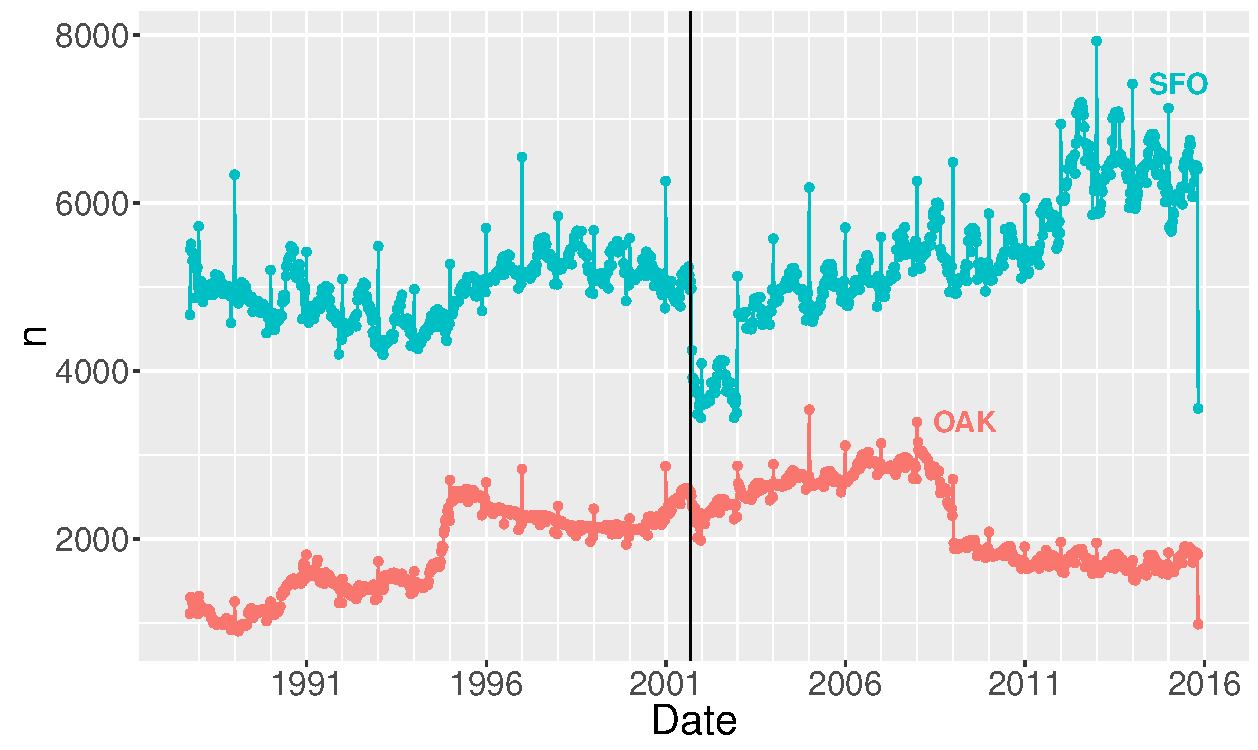
\includegraphics[width = \figurewidth]{figure/SanFran_Flights_by_date-1}}
\caption{Number of depatures over time from Oakland and San Francisco Intl.}
\end{figure}

\begin{knitrout}
\definecolor{shadecolor}{rgb}{0.969, 0.969, 0.969}\color{fgcolor}\begin{kframe}
\begin{alltt}
\hlstd{carriers} \hlkwb{<-} \hlkwd{as.data.table}\hlstd{(airlines)}
\hlkwa{if}\hlstd{(}\hlstr{"carrier"} \hlopt \hlkwd{names}\hlstd{(carriers))}
  \hlkwd{setnames}\hlstd{(carriers,} \hlkwc{old} \hlstd{=} \hlstr{"carrier"}\hlstd{,} \hlkwc{new} \hlstd{=} \hlstr{"UniqueCarrier"}\hlstd{)}

\hlkwd{setkey}\hlstd{(carriers, UniqueCarrier)}
\hlkwd{set}\hlstd{(carriers,} \hlkwc{j} \hlstd{=} \hlnum{1L}\hlstd{,} \hlkwc{value} \hlstd{=} \hlkwd{as.character}\hlstd{(carriers[[}\hlnum{1L}\hlstd{]]))}
\hlkwd{set}\hlstd{(carriers,} \hlkwc{j} \hlstd{=} \hlnum{2L}\hlstd{,} \hlkwc{value} \hlstd{=} \hlkwd{gsub}\hlstd{(}\hlstr{"^([A-Za-z]+)\textbackslash{}\textbackslash{}s.*$"}\hlstd{,} \hlstr{"\textbackslash{}\textbackslash{}1"}\hlstd{, carriers[[}\hlnum{2L}\hlstd{]]))}

\hlstd{flightsSanFran} \hlopt
  \hlkwd{filter}\hlstd{(Origin} \hlopt \hlkwd{c}\hlstd{(}\hlstr{"SFO"}\hlstd{,} \hlstr{"OAK"}\hlstd{))} \hlopt
  \hlkwd{count}\hlstd{(Year, Month, Origin, UniqueCarrier)} \hlopt
  \hlkwd{group_by}\hlstd{(UniqueCarrier)} \hlopt
  \hlkwd{filter}\hlstd{(}\hlkwd{sum}\hlstd{(n)} \hlopt{>} \hlstd{(}\hlnum{2015} \hlopt{-} \hlnum{1987}\hlstd{)} \hlopt{*} \hlnum{12} \hlopt{*} \hlnum{30}\hlstd{)}  \hlopt
  \hlkwd{mutate}\hlstd{(}\hlkwc{Date} \hlstd{= Year} \hlopt{+} \hlstd{(Month} \hlopt{-} \hlnum{1}\hlstd{)}\hlopt{/}\hlnum{12}\hlstd{)} \hlopt
  \hlkwd{setkey}\hlstd{(UniqueCarrier)} \hlopt
  \hlkwd{merge}\hlstd{(carriers)} \hlopt
  \hlkwd{ggplot}\hlstd{(}\hlkwd{aes}\hlstd{(}\hlkwc{x} \hlstd{= Date,} \hlkwc{y} \hlstd{= n} \hlopt{*} \hlstd{sample.weight.int,} \hlkwc{color} \hlstd{= name,} \hlkwc{group} \hlstd{=} \hlkwd{interaction}\hlstd{(name,Origin)))} \hlopt{+} \hlkwd{ylab}\hlstd{(}\hlstr{"Number of departures"}\hlstd{)} \hlopt{+}
  \hlkwd{geom_smooth}\hlstd{(}\hlkwc{span} \hlstd{=} \hlnum{0.25}\hlstd{,} \hlkwc{se} \hlstd{=} \hlnum{FALSE}\hlstd{)} \hlopt{+}
  \hlkwd{geom_text}\hlstd{(}\hlkwd{aes}\hlstd{(}\hlkwc{label} \hlstd{=} \hlkwd{ifelse}\hlstd{(Date} \hlopt{==} \hlkwd{max}\hlstd{(Date),}
                               \hlstd{name,}
                               \hlnum{NA_character_}\hlstd{),}
                \hlkwc{vjust} \hlstd{=} \hlkwd{ifelse}\hlstd{(name} \hlopt{==} \hlstr{"Southwest"} \hlopt{&} \hlstd{Origin} \hlopt{==} \hlstr{"SFO"}\hlstd{,}
                                 \hlopt{-}\hlnum{0.5}\hlstd{,}
                                 \hlnum{0.5}\hlstd{)),}
            \hlkwc{nudge_x} \hlstd{=} \hlnum{0.75}\hlstd{,}
            \hlkwc{size} \hlstd{=} \hlnum{5}\hlstd{)} \hlopt{+} \hlkwd{theme}\hlstd{(}\hlkwc{legend.position} \hlstd{=} \hlstr{"none"}\hlstd{)} \hlopt{+}
  \hlkwd{annotate}\hlstd{(}\hlstr{"blank"}\hlstd{,} \hlkwc{x} \hlstd{=} \hlnum{2019}\hlstd{,} \hlkwc{y} \hlstd{=} \hlnum{0}\hlstd{)} \hlopt{+}
  \hlkwd{facet_grid}\hlstd{(Origin} \hlopt{~} \hlstd{.)} \hlopt{+}
  \hlkwd{theme}\hlstd{(}\hlkwc{text} \hlstd{=} \hlkwd{element_text}\hlstd{(}\hlkwc{size} \hlstd{=} \hlnum{16}\hlstd{))}
\end{alltt}


{\ttfamily\noindent\color{warningcolor}{\#\# Warning in simpleLoess(y, x, w, span, degree = degree, parametric = parametric, : span too small.\ \  fewer data values than degrees of freedom.}}

{\ttfamily\noindent\color{warningcolor}{\#\# Warning in simpleLoess(y, x, w, span, degree = degree, parametric = parametric, : pseudoinverse used at 2002.1}}

{\ttfamily\noindent\color{warningcolor}{\#\# Warning in simpleLoess(y, x, w, span, degree = degree, parametric = parametric, : neighborhood radius 0.17125}}

{\ttfamily\noindent\color{warningcolor}{\#\# Warning in simpleLoess(y, x, w, span, degree = degree, parametric = parametric, : reciprocal condition number\ \ 0}}

{\ttfamily\noindent\color{warningcolor}{\#\# Warning in simpleLoess(y, x, w, span, degree = degree, parametric = parametric, : There are other near singularities as well. 0.029327}}

{\ttfamily\noindent\color{warningcolor}{\#\# Warning: Removed 4579 rows containing missing values (geom\_text).}}\end{kframe}
\end{knitrout}
\begin{figure}
\centering
{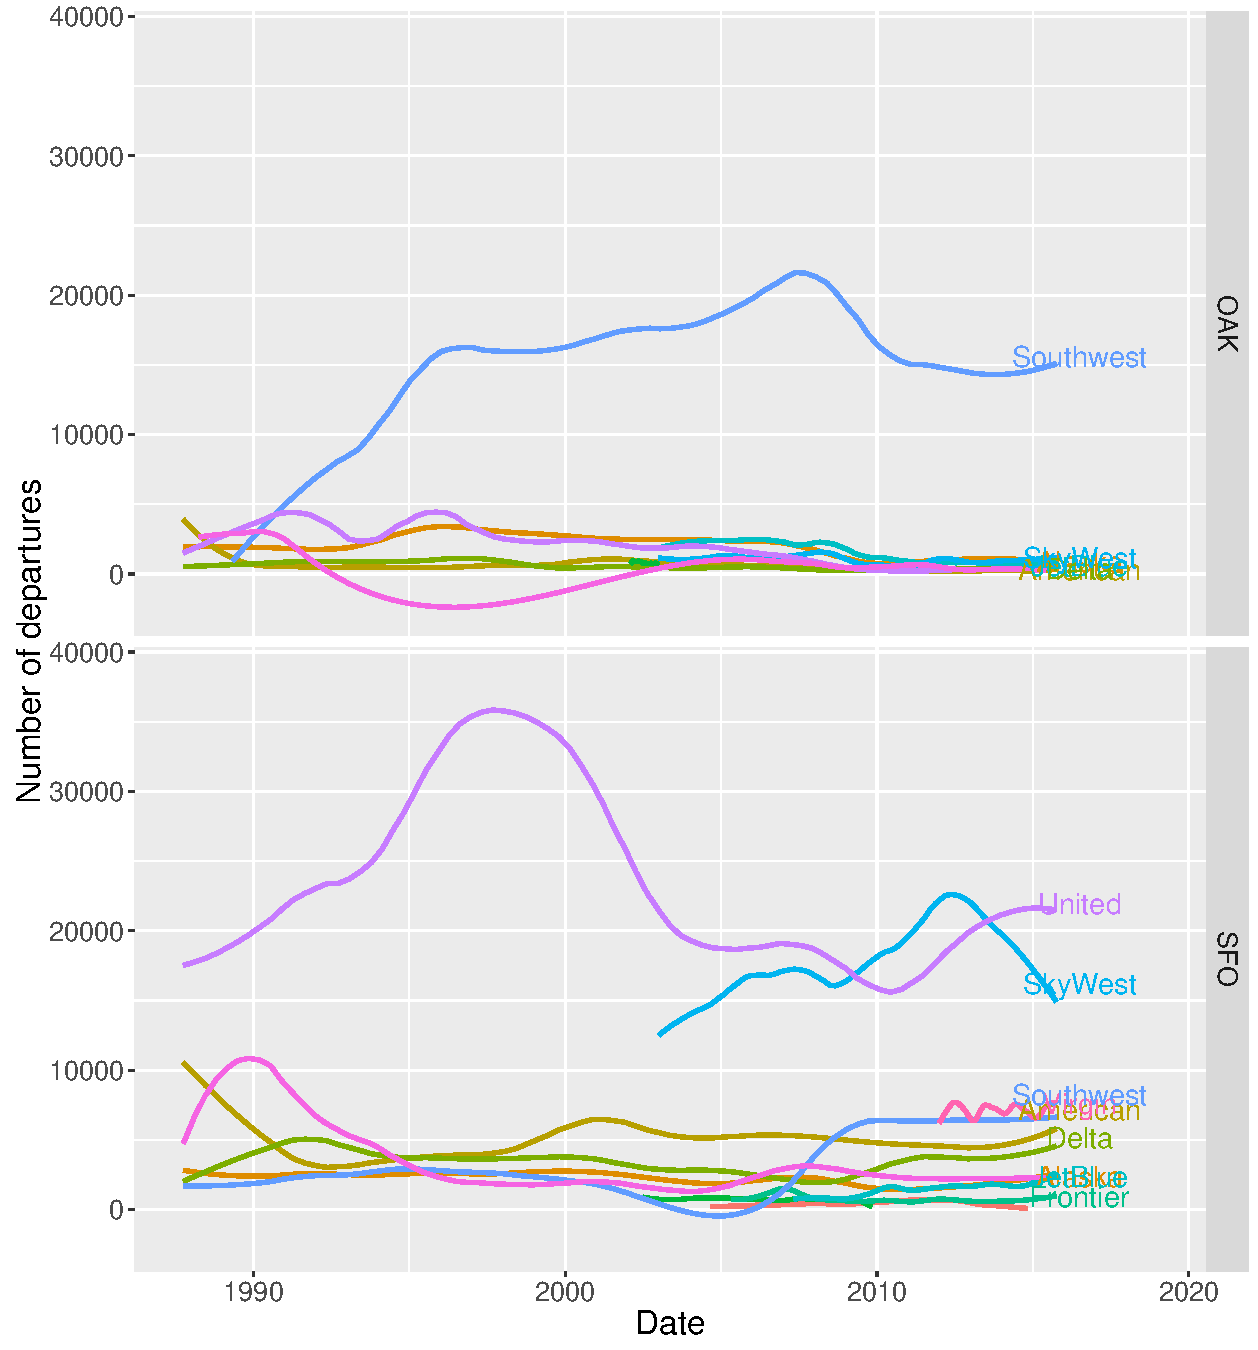
\includegraphics[width = \figurewidth]{figure/SanFran_Flights_by_Carrier-1}}
\caption{Number of depatures over time from Oakland and San Francisco Intl.}
\end{figure}

After September 11, flights from SFO fell, whereas OAK's volume did notFlights fell more in SFO than they did in OAK because most of OAK's flights are from Southwest, which did not change its flight patterns. Furthermore, United was affected more than most airlines from the aftermath of the attacks.

\begin{knitrout}
\definecolor{shadecolor}{rgb}{0.969, 0.969, 0.969}\color{fgcolor}\begin{kframe}
\begin{alltt}
\hlstd{top_5_carriers} \hlkwb{<-}
  \hlstd{flights} \hlopt
  \hlkwd{count}\hlstd{(UniqueCarrier)} \hlopt
  \hlkwd{arrange}\hlstd{(}\hlkwd{desc}\hlstd{(n))} \hlopt
  \hlkwd{mutate}\hlstd{(}\hlkwc{TopN} \hlstd{=} \hlnum{1}\hlopt{:}\hlkwd{n}\hlstd{()} \hlopt{<=} \hlnum{5}\hlstd{)} \hlopt
  \hlkwd{mutate}\hlstd{(}\hlkwc{Carrier_other} \hlstd{=} \hlkwd{ifelse}\hlstd{(TopN, UniqueCarrier,} \hlstr{"Other"}\hlstd{))} \hlopt
  \hlkwd{select}\hlstd{(}\hlopt{-}\hlstd{n)} \hlopt
  \hlkwd{setkey}\hlstd{(UniqueCarrier)}

\hlstd{flights} \hlopt
  \hlkwd{setkey}\hlstd{(UniqueCarrier)} \hlopt
  \hlkwd{merge}\hlstd{(top_5_carriers)} \hlopt
  \hlkwd{count}\hlstd{(Carrier_other, Year)} \hlopt
  \hlkwd{ggplot}\hlstd{(}\hlkwd{aes}\hlstd{(}\hlkwc{x} \hlstd{= Year,} \hlkwc{y} \hlstd{= n} \hlopt{*} \hlstd{sample.weight.int,} \hlkwc{color} \hlstd{= Carrier_other,} \hlkwc{group} \hlstd{= Carrier_other))} \hlopt{+}
  \hlkwd{geom_line}\hlstd{()} \hlopt{+}
  \hlkwd{scale_colour_brewer}\hlstd{(}\hlkwc{palette} \hlstd{=} \hlstr{"Accent"}\hlstd{)} \hlopt{+}
  \hlkwd{scale_y_continuous}\hlstd{(}\hlkwc{label} \hlstd{= scales}\hlopt{::}\hlstd{comma)}
\end{alltt}
\end{kframe}
\end{knitrout}
\begin{figure}
{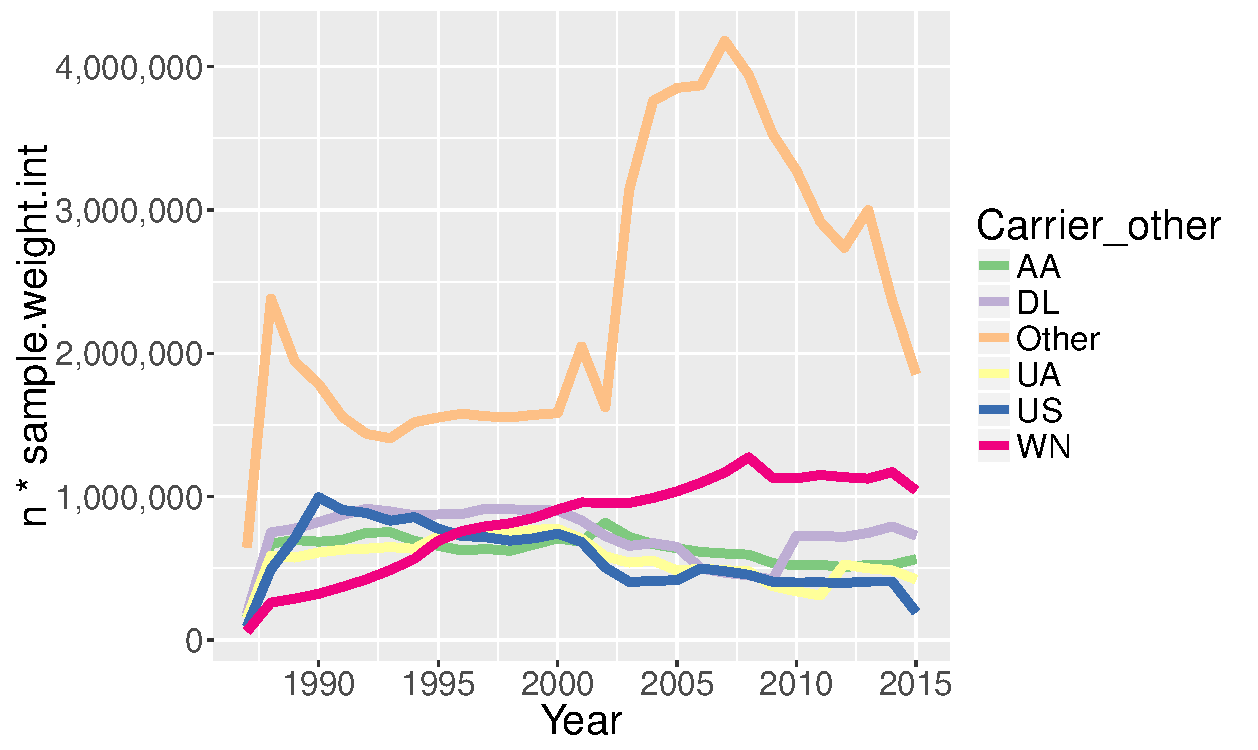
\includegraphics[width=\figurewidth]{figure/Volume-by-Carrier-1}}
\end{figure}

\begin{knitrout}
\definecolor{shadecolor}{rgb}{0.969, 0.969, 0.969}\color{fgcolor}\begin{kframe}
\begin{alltt}
\hlstd{majorAirportThreshold} \hlkwb{=} \hlnum{10}

\hlstd{major_airports} \hlkwb{<-}
  \hlstd{flights[ ,}\hlkwd{.}\hlstd{(}\hlkwc{n} \hlstd{= .N),} \hlkwc{by} \hlstd{= Dest][}\hlkwd{order}\hlstd{(}\hlopt{-}\hlstd{n)]} \hlopt \hlcom{# flights %>% count(Dest) %>% arrange(desc(n))}
  \hlkwd{mutate}\hlstd{(}\hlkwc{TopN} \hlstd{=} \hlnum{1}\hlopt{:}\hlkwd{n}\hlstd{()} \hlopt{<=} \hlstd{majorAirportThreshold)} \hlopt
  \hlkwd{mutate}\hlstd{(}\hlkwc{AirportOther} \hlstd{=} \hlkwd{ifelse}\hlstd{(TopN, Dest,} \hlstr{"Other_airport"}\hlstd{))} \hlopt
  \hlkwd{select}\hlstd{(}\hlopt{-}\hlstd{n)} \hlopt
  \hlkwd{setkey}\hlstd{(Dest)}

\hlstd{airports_by_volume_by_year} \hlkwb{<-} \hlstd{flights[major_airports][ ,}\hlkwd{.}\hlstd{(}\hlkwc{n} \hlstd{= .N} \hlopt{*} \hlstd{sample.weight.int),} \hlkwc{by} \hlstd{=} \hlkwd{list}\hlstd{(Year, AirportOther)]}

\hlstd{airports_by_volume_by_2014} \hlkwb{<-}
  \hlstd{airports_by_volume_by_year} \hlopt
  \hlkwd{filter}\hlstd{(Year} \hlopt{==} \hlnum{2014}\hlstd{)} \hlopt
  \hlkwd{filter}\hlstd{(AirportOther} \hlopt{!=} \hlstr{"AirportOther"}\hlstd{)} \hlopt
  \hlkwd{merge}\hlstd{(}\hlkwd{select}\hlstd{(nycflights.airports, faa, name),} \hlkwc{by.x} \hlstd{=} \hlstr{"AirportOther"}\hlstd{,} \hlkwc{by.y} \hlstd{=} \hlstr{"faa"}\hlstd{)} \hlopt
  \hlkwd{arrange}\hlstd{(}\hlkwd{desc}\hlstd{(n))}
\hlkwd{gc}\hlstd{(}\hlnum{0}\hlstd{,}\hlnum{1}\hlstd{)}
\end{alltt}
\begin{verbatim}
##              used   (Mb) gc trigger    (Mb)   max used   (Mb)
## Ncells     695285   37.2    1867598    99.8     695285   37.2
## Vcells 1290767501 9847.8 3617730857 27601.1 1290767501 9847.8
\end{verbatim}
\begin{alltt}
\hlkwd{setkey}\hlstd{(flights, Dest)}
\hlkwd{gc}\hlstd{(}\hlnum{0}\hlstd{,}\hlnum{1}\hlstd{)}
\end{alltt}
\begin{verbatim}
##              used   (Mb) gc trigger    (Mb)   max used   (Mb)
## Ncells     695181   37.2    1867598    99.8     695181   37.2
## Vcells 1290762564 9847.8 3617730857 27601.1 1290762564 9847.8
\end{verbatim}
\begin{alltt}
\hlstd{airports_by_volume_by_year} \hlopt
  \hlkwd{filter}\hlstd{(AirportOther} \hlopt{!=} \hlstr{"Other_airport"}\hlstd{, Year} \hlopt{>} \hlnum{1987L}\hlstd{, Year} \hlopt{<} \hlnum{2015L}\hlstd{)}  \hlopt
  \hlkwd{merge}\hlstd{(}\hlkwd{select}\hlstd{(nycflights.airports, faa, name),} \hlkwc{by.x} \hlstd{=} \hlstr{"AirportOther"}\hlstd{,} \hlkwc{by.y} \hlstd{=} \hlstr{"faa"}\hlstd{)} \hlopt
  \hlkwd{mutate}\hlstd{(}\hlkwc{name} \hlstd{=} \hlkwd{factor}\hlstd{(name,} \hlkwc{levels} \hlstd{= airports_by_volume_by_2014}\hlopt{$}\hlstd{name))} \hlopt
  \hlkwd{ggplot}\hlstd{(}\hlkwd{aes}\hlstd{(}\hlkwc{x} \hlstd{= Year,} \hlkwc{y} \hlstd{= n,} \hlkwc{group} \hlstd{= name,} \hlkwc{color} \hlstd{= name))} \hlopt{+}
  \hlkwd{geom_line}\hlstd{()}
\hlkwd{gc}\hlstd{(}\hlnum{0}\hlstd{,}\hlnum{1}\hlstd{)}
\end{alltt}
\begin{verbatim}
##              used   (Mb) gc trigger    (Mb)   max used   (Mb)
## Ncells     702432   37.6    1867598    99.8     702432   37.6
## Vcells 1290783051 9847.9 3617730857 27601.1 1290783051 9847.9
\end{verbatim}
\end{kframe}
\end{knitrout}

\begin{knitrout}
\definecolor{shadecolor}{rgb}{0.969, 0.969, 0.969}\color{fgcolor}\begin{kframe}
\begin{alltt}
\hlstd{rel_vol_major_airports} \hlkwb{<-}
  \hlstd{flights[major_airports][ ,}\hlkwd{.}\hlstd{(}\hlkwc{n} \hlstd{= .N} \hlopt{*} \hlstd{sample.weight.int),} \hlkwc{by} \hlstd{=} \hlkwd{list}\hlstd{(Year, AirportOther)]} \hlopt
  \hlkwd{filter}\hlstd{(AirportOther} \hlopt{!=} \hlstr{"Other_airport"}\hlstd{, Year} \hlopt{>} \hlnum{1987L}\hlstd{, Year} \hlopt{<} \hlnum{2015L}\hlstd{)} \hlopt
  \hlkwd{arrange}\hlstd{(Year)} \hlopt
  \hlkwd{group_by}\hlstd{(AirportOther)} \hlopt
  \hlkwd{mutate}\hlstd{(}\hlkwc{rel} \hlstd{= n}\hlopt{/}\hlkwd{first}\hlstd{(n))} \hlopt
  \hlkwd{merge}\hlstd{(}\hlkwd{select}\hlstd{(nycflights.airports, faa, name),} \hlkwc{by.x} \hlstd{=} \hlstr{"AirportOther"}\hlstd{,} \hlkwc{by.y} \hlstd{=} \hlstr{"faa"}\hlstd{)}

\hlstd{last_values} \hlkwb{<-}
  \hlstd{rel_vol_major_airports} \hlopt
  \hlkwd{filter}\hlstd{(Year} \hlopt{==} \hlkwd{max}\hlstd{(Year))} \hlopt
  \hlkwd{arrange}\hlstd{(rel)}

\hlstd{rel_vol_major_airports}  \hlopt
  \hlkwd{mutate}\hlstd{(}\hlkwc{name} \hlstd{=} \hlkwd{factor}\hlstd{(name,} \hlkwc{levels} \hlstd{=} \hlkwd{rev}\hlstd{(last_values}\hlopt{$}\hlstd{name)))} \hlopt
  \hlkwd{ggplot}\hlstd{(}\hlkwd{aes}\hlstd{(}\hlkwc{x} \hlstd{= Year,} \hlkwc{y} \hlstd{= rel,} \hlkwc{group} \hlstd{= name,} \hlkwc{color} \hlstd{= name))} \hlopt{+}
  \hlkwd{geom_line}\hlstd{()}
\end{alltt}
\end{kframe}
\end{knitrout}
\begin{figure}
{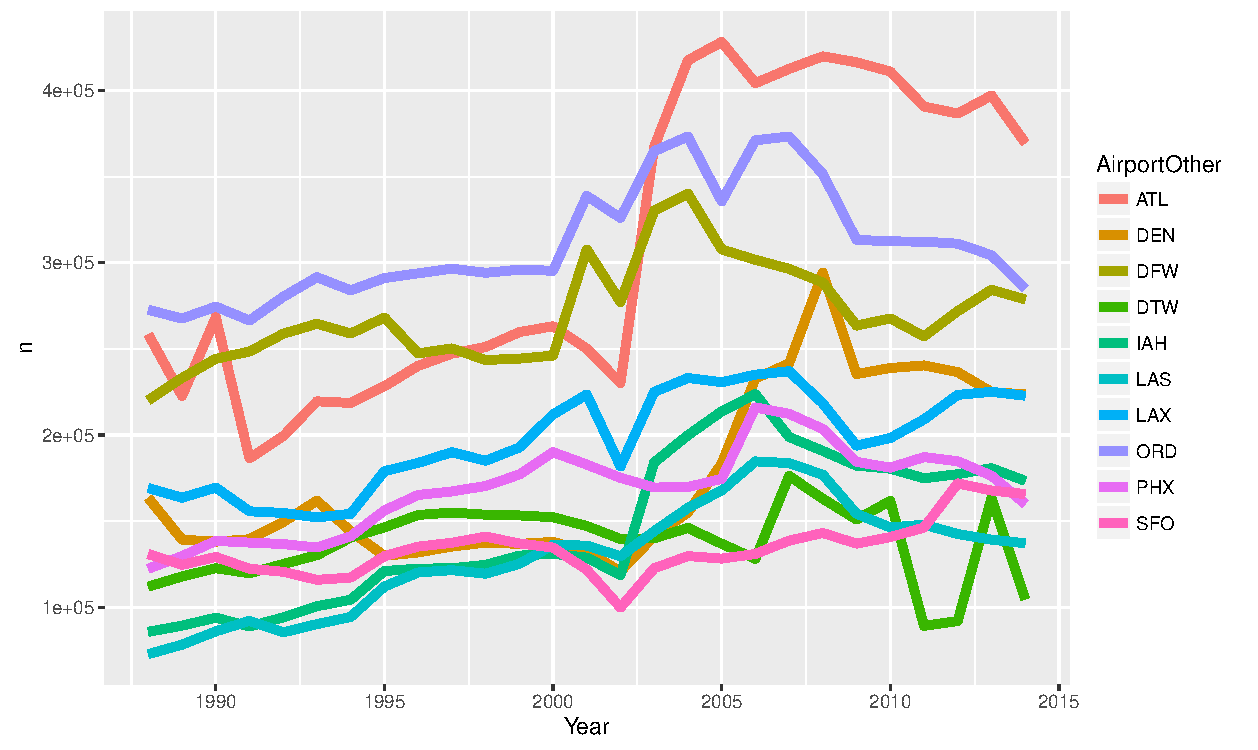
\includegraphics[width=\figurewidth]{figure/Volume-by-major-airports-1}}
\caption{Annual flights by the top 10 airports by total volume.}
\end{figure}

\begin{figure}
{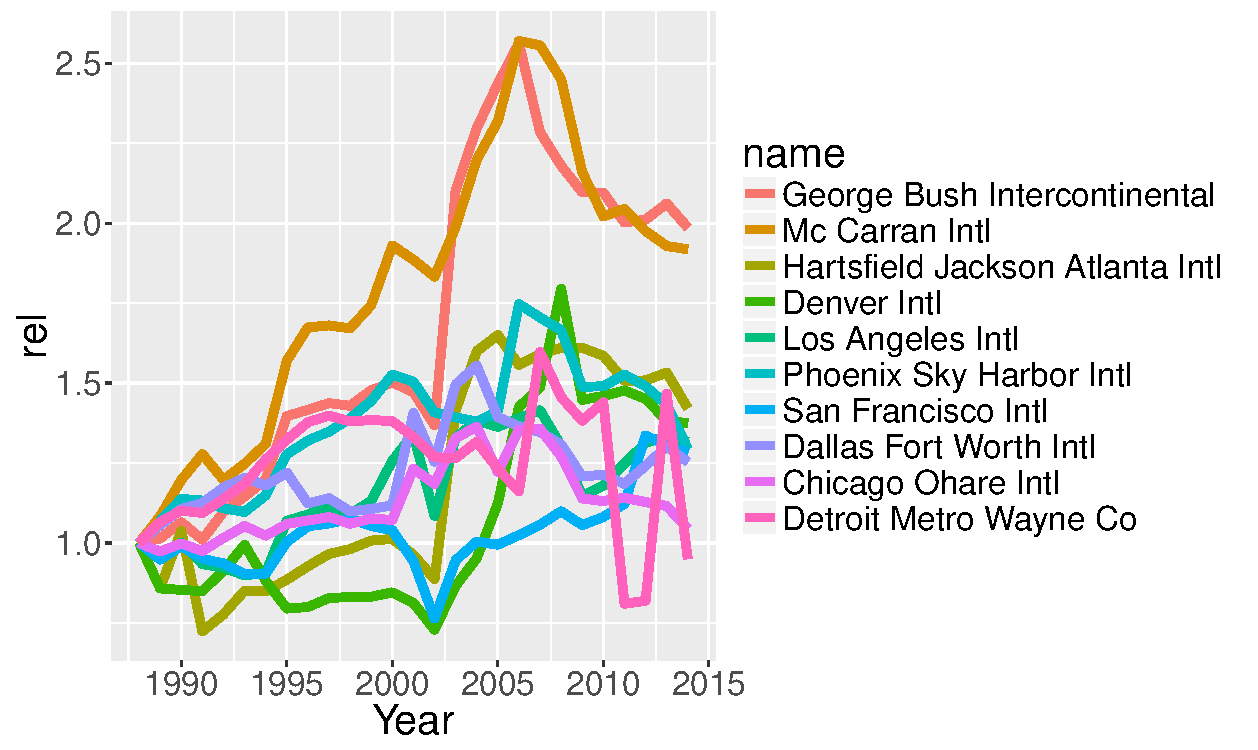
\includegraphics[width=\figurewidth]{figure/Relative-volume-by-major-airports-1}}
\caption{Annual flights by airport, 1988 = 1.}
\end{figure}

\begin{knitrout}
\definecolor{shadecolor}{rgb}{0.969, 0.969, 0.969}\color{fgcolor}\begin{kframe}
\begin{alltt}
\hlstd{otp201510} \hlkwb{<-}
  \hlkwd{fread}\hlstd{(}\hlstr{"../dep_delay/On_Time_On_Time_Performance_2015_10.csv"}\hlstd{)}
\end{alltt}
\begin{verbatim}
## 
Read 43.2% of 486165 rows
Read 78.2% of 486165 rows
Read 486165 rows and 110 (of 110) columns from 0.204 GB file in 00:00:04
\end{verbatim}
\begin{alltt}
\hlstd{city_decoder} \hlkwb{<-}
  \hlstd{otp201510} \hlopt
  \hlkwd{select}\hlstd{(}\hlkwd{contains}\hlstd{(}\hlstr{"Origin"}\hlstd{))} \hlopt
  \hlstd{unique}

\hlkwd{setkey}\hlstd{(city_decoder, OriginCityMarketID)}

\hlkwd{gc}\hlstd{(T,T)}
\end{alltt}
\begin{verbatim}
##              used    (Mb) gc trigger    (Mb)   max used    (Mb)
## Ncells     708733    37.9    1867598    99.8     708733    37.9
## Vcells 1335752294 10191.0 3617730857 27601.1 1335752294 10191.0
\end{verbatim}
\begin{alltt}
\hlstd{city_market_decoder} \hlkwb{<-}
  \hlkwd{fread}\hlstd{(}\hlstr{"../metadata//L_CITY_MARKET_ID.csv"}\hlstd{)} \hlopt
  \hlkwd{setnames}\hlstd{(}\hlkwc{old} \hlstd{=} \hlkwd{c}\hlstd{(}\hlstr{"Code"}\hlstd{,} \hlstr{"Description"}\hlstd{),}
           \hlkwc{new} \hlstd{=} \hlkwd{c}\hlstd{(}\hlstr{"OriginCityMarketID"}\hlstd{,} \hlstr{"OriginCityMarketDescription"}\hlstd{))} \hlopt
  \hlkwd{setkey}\hlstd{(OriginCityMarketID)}
\hlstd{city_market_decoder[,OriginCityMarketID} \hlkwb{:=} \hlkwd{as.integer}\hlstd{(OriginCityMarketID)]}
\hlstd{city_decoder} \hlkwb{<-} \hlkwd{merge}\hlstd{(city_decoder, city_market_decoder,} \hlkwc{by} \hlstd{=} \hlstr{"OriginCityMarketID"}\hlstd{,} \hlkwc{all.x} \hlstd{=} \hlnum{TRUE}\hlstd{,} \hlkwc{all.y} \hlstd{=} \hlnum{FALSE}\hlstd{)}
\hlkwd{gc}\hlstd{(T,T)}
\end{alltt}
\begin{verbatim}
##              used    (Mb) gc trigger    (Mb)   max used    (Mb)
## Ncells     714266    38.2    1867598    99.8     714266    38.2
## Vcells 1335778567 10191.2 3617730857 27601.1 1335778567 10191.2
\end{verbatim}
\end{kframe}
\end{knitrout}

\begin{knitrout}
\definecolor{shadecolor}{rgb}{0.969, 0.969, 0.969}\color{fgcolor}\begin{kframe}
\begin{alltt}
\hlstd{market_volume_by_year} \hlkwb{<-}
  \hlstd{flightsSanFran} \hlopt
  \hlkwd{filter}\hlstd{(Dest} \hlopt \hlkwd{c}\hlstd{(}\hlstr{"SFO"}\hlstd{,} \hlstr{"OAK"}\hlstd{))} \hlopt
  \hlkwd{merge}\hlstd{(city_decoder,} \hlkwc{by} \hlstd{=} \hlstr{"Origin"}\hlstd{)} \hlopt
  \hlkwd{count}\hlstd{(Year, OriginCityMarketDescription)} \hlopt
  \hlkwd{mutate}\hlstd{(}\hlkwc{State} \hlstd{=} \hlkwd{gsub}\hlstd{(}\hlstr{"^.*([A-Z]\{2\}).*$"}\hlstd{,} \hlstr{"\textbackslash{}\textbackslash{}1"}\hlstd{, OriginCityMarketDescription))} \hlopt
  \hlkwd{filter}\hlstd{(n} \hlopt{>} \hlnum{3650}\hlstd{)} \hlopt
  \hlkwd{mutate}\hlstd{(}\hlkwc{Label} \hlstd{=} \hlkwd{ifelse}\hlstd{(Year} \hlopt{==} \hlkwd{max}\hlstd{(Year), OriginCityMarketDescription,} \hlnum{NA_character_}\hlstd{))} \hlopt
  \hlkwd{arrange}\hlstd{(Year,} \hlkwd{desc}\hlstd{(n))}

\hlstd{mkt.vol.by.yr} \hlkwb{<-} \hlkwa{function}\hlstd{(}\hlkwc{year}\hlstd{,} \hlkwc{colname}\hlstd{)\{}
  \hlstd{magrittr}\hlopt{::}\hlkwd{extract2}\hlstd{(dplyr}\hlopt{::}\hlkwd{filter}\hlstd{(market_volume_by_year, Year} \hlopt{==} \hlstd{year), colname)}
\hlstd{\}}
\hlstd{market_volume_by_year} \hlopt
  \hlkwd{mutate}\hlstd{(}\hlkwc{OriginCityMarketDescription} \hlstd{=} \hlkwd{factor}\hlstd{(OriginCityMarketDescription,} \hlkwc{levels} \hlstd{=} \hlkwd{mkt.vol.by.yr}\hlstd{(}\hlnum{2015}\hlstd{,} \hlstr{"OriginCityMarketDescription"}\hlstd{)))} \hlopt
  \hlkwd{ggplot}\hlstd{(}\hlkwd{aes}\hlstd{(}\hlkwc{x} \hlstd{= Year,} \hlkwc{y} \hlstd{= n,} \hlkwc{color} \hlstd{= OriginCityMarketDescription,} \hlkwc{group} \hlstd{= OriginCityMarketDescription))} \hlopt{+}
  \hlcom{#facet_grid(State ~ .) + }
  \hlkwd{geom_line}\hlstd{()} \hlopt{+}
  \hlcom{#geom_text(aes(label = Label)) + }
  \hlcom{#geom_dl(method = list("top.points", dl.trans(y = y+0.25), fontfamily = "bold"), aes(label = OriginCityMarketDescription)) + }
  \hlkwd{theme}\hlstd{(}\hlkwc{legend.position} \hlstd{=} \hlstr{"none"}\hlstd{)} \hlkwb{->} \hlstd{p}
\hlkwd{direct.label}\hlstd{(p,} \hlkwd{list}\hlstd{(}\hlstr{"top.points"}\hlstd{,} \hlkwd{dl.trans}\hlstd{(}\hlkwc{y} \hlstd{= y}\hlopt{+}\hlnum{0.25}\hlstd{),} \hlkwc{fontface}\hlstd{=}\hlstr{"bold"}\hlstd{))}
\end{alltt}
\end{kframe}
\end{knitrout}



\begin{knitrout}
\definecolor{shadecolor}{rgb}{0.969, 0.969, 0.969}\color{fgcolor}\begin{kframe}
\begin{alltt}
\hlstd{FAA_aircraft} \hlkwb{<-}
  \hlkwd{fread}\hlstd{(}\hlstr{"../metadata/planes.csv"}\hlstd{)} \hlopt
  \hlkwd{setnames}\hlstd{(}\hlkwc{old} \hlstd{=} \hlkwd{c}\hlstd{(}\hlstr{"tailnum"}\hlstd{,} \hlstr{"year"}\hlstd{),} \hlkwc{new} \hlstd{=} \hlkwd{c}\hlstd{(}\hlstr{"TailNum"}\hlstd{,} \hlstr{"YearOfReg"}\hlstd{))} \hlopt
  \hlkwd{setkey}\hlstd{(TailNum)}
\end{alltt}
\end{kframe}
\end{knitrout}

\begin{knitrout}
\definecolor{shadecolor}{rgb}{0.969, 0.969, 0.969}\color{fgcolor}\begin{kframe}
\begin{alltt}
\hlstd{flights} \hlopt
  \hlkwd{group_by}\hlstd{(Origin, Dest)} \hlopt
  \hlkwd{filter}\hlstd{(}\hlkwd{n}\hlstd{()} \hlopt{>} \hlnum{50000}\hlstd{)} \hlopt
  \hlkwd{mutate}\hlstd{(}\hlkwc{Route} \hlstd{=} \hlkwd{paste0}\hlstd{(Origin,} \hlstr{"-"}\hlstd{, Dest),}
         \hlkwc{RevRoute} \hlstd{=} \hlkwd{paste0}\hlstd{(Dest,} \hlstr{"-"}\hlstd{, Origin),}
         \hlkwc{maxRoute} \hlstd{=} \hlkwd{pmax}\hlstd{(Route, RevRoute))} \hlopt
  \hlkwd{ggplot}\hlstd{(}\hlkwd{aes}\hlstd{(}\hlkwc{x} \hlstd{= ActualElapsedTime))} \hlopt{+}
  \hlkwd{geom_density}\hlstd{(}\hlkwd{aes}\hlstd{(}\hlkwc{fill} \hlstd{= maxRoute),} \hlkwc{alpha} \hlstd{=} \hlnum{0.5}\hlstd{)} \hlopt{+} \hlkwd{xlim}\hlstd{(}\hlnum{0}\hlstd{,}\hlnum{300}\hlstd{)}
\end{alltt}


{\ttfamily\noindent\color{warningcolor}{\#\# Warning: Removed 1193422 rows containing non-finite values (stat\_density).}}\end{kframe}
\end{knitrout}

\begin{knitrout}
\definecolor{shadecolor}{rgb}{0.969, 0.969, 0.969}\color{fgcolor}\begin{kframe}
\begin{alltt}
\hlstd{flights} \hlopt
  \hlkwd{select}\hlstd{(Origin, Dest, ActualElapsedTime)} \hlopt
  \hlkwd{group_by}\hlstd{(Origin, Dest)} \hlopt
  \hlkwd{summarise}\hlstd{(}\hlkwc{average_time} \hlstd{=} \hlkwd{mean}\hlstd{(ActualElapsedTime,} \hlkwc{na.rm} \hlstd{=} \hlnum{TRUE}\hlstd{),}
            \hlkwc{sd_time} \hlstd{=} \hlkwd{sd}\hlstd{(ActualElapsedTime,} \hlkwc{na.rm} \hlstd{=} \hlnum{TRUE}\hlstd{),}
            \hlkwc{n} \hlstd{=} \hlkwd{n}\hlstd{())} \hlopt
  \hlkwd{mutate}\hlstd{(}\hlkwc{avg_less_sd} \hlstd{= (sd_time} \hlopt{-} \hlstd{average_time)} \hlopt{/} \hlstd{average_time)} \hlopt
  \hlkwd{arrange}\hlstd{(avg_less_sd)} \hlopt
  \hlkwd{mutate}\hlstd{(}\hlkwc{Route} \hlstd{=} \hlkwd{paste0}\hlstd{(Origin,} \hlstr{"-"}\hlstd{, Dest),}
         \hlkwc{Label} \hlstd{=} \hlkwd{ifelse}\hlstd{(Route} \hlopt \hlkwd{c}\hlstd{(}\hlstr{'ROC-JFK'}\hlstd{,} \hlstr{'SLC-PHX'}\hlstd{,} \hlstr{'DCA-LGA'}\hlstd{,} \hlstr{'ORD-EWR'}\hlstd{), Route,} \hlnum{NA_character_}\hlstd{),}
         \hlkwc{hasLabel} \hlstd{=} \hlopt{!}\hlkwd{is.na}\hlstd{(Label))} \hlopt
  \hlkwd{ggplot}\hlstd{(}\hlkwd{aes}\hlstd{(}\hlkwc{x} \hlstd{= average_time,} \hlkwc{y} \hlstd{= sd_time))} \hlopt{+}
  \hlcom{#geom_point(aes(alpha = n/max(n))) + scale_alpha_identity() + }
  \hlkwd{geom_point}\hlstd{(}\hlkwd{aes}\hlstd{(}\hlkwc{size} \hlstd{= n,} \hlkwc{fill} \hlstd{= hasLabel,} \hlkwc{alpha} \hlstd{= hasLabel),} \hlkwc{color} \hlstd{=} \hlstr{"black"}\hlstd{,} \hlkwc{stroke} \hlstd{=} \hlnum{1}\hlstd{,} \hlkwc{shape} \hlstd{=} \hlnum{21}\hlstd{)} \hlopt{+} \hlkwd{scale_size_area}\hlstd{(}\hlkwc{max_size} \hlstd{=} \hlnum{10}\hlstd{)} \hlopt{+}
  \hlkwd{scale_fill_manual}\hlstd{(}\hlkwc{values} \hlstd{=} \hlkwd{c}\hlstd{(Orange,} \hlstr{"red"}\hlstd{))}  \hlopt{+}
  \hlkwd{scale_alpha_manual}\hlstd{(}\hlkwc{values} \hlstd{=} \hlkwd{c}\hlstd{(}\hlnum{0.5}\hlstd{,} \hlnum{1}\hlstd{))} \hlopt{+}
  \hlkwd{geom_text}\hlstd{(}\hlkwd{aes}\hlstd{(}\hlkwc{label} \hlstd{= Label),} \hlkwc{color} \hlstd{=} \hlstr{"red"}\hlstd{,} \hlkwc{fontface} \hlstd{=} \hlstr{"bold"}\hlstd{,} \hlkwc{hjust} \hlstd{=} \hlnum{1.1}\hlstd{,} \hlkwc{vjust} \hlstd{=} \hlnum{0.0}\hlstd{,} \hlkwc{nudge_x} \hlstd{=} \hlopt{-}\hlnum{1}\hlstd{,} \hlkwc{nudge_y} \hlstd{=} \hlnum{0.2}\hlstd{)} \hlopt{+}
  \hlkwd{coord_cartesian}\hlstd{(}\hlkwc{xlim} \hlstd{=} \hlkwd{c}\hlstd{(}\hlnum{0}\hlstd{,}\hlnum{480}\hlstd{),} \hlkwc{ylim} \hlstd{=} \hlkwd{c}\hlstd{(}\hlnum{0}\hlstd{,}\hlnum{50}\hlstd{))} \hlopt{+}
  \hlkwd{scale_x_continuous}\hlstd{(}\hlstr{"Average elapsed time"}\hlstd{,} \hlkwc{expand} \hlstd{=} \hlkwd{c}\hlstd{(}\hlnum{0}\hlstd{,}\hlnum{0}\hlstd{))} \hlopt{+}
  \hlkwd{scale_y_continuous}\hlstd{(}\hlstr{"SD of time"}\hlstd{,} \hlkwc{expand} \hlstd{=} \hlkwd{c}\hlstd{(}\hlnum{0}\hlstd{,}\hlnum{0}\hlstd{))}
\end{alltt}


{\ttfamily\noindent\color{warningcolor}{\#\# Warning: Removed 886 rows containing missing values (geom\_point).}}

{\ttfamily\noindent\color{warningcolor}{\#\# Warning: Removed 8792 rows containing missing values (geom\_text).}}\end{kframe}
\end{knitrout}


\section{Effect of 9-11}
\begin{knitrout}
\definecolor{shadecolor}{rgb}{0.969, 0.969, 0.969}\color{fgcolor}\begin{kframe}
\begin{alltt}
\hlstd{flights} \hlopt
  \hlkwd{group_by}\hlstd{(Year, Month, DayofMonth)} \hlopt
  \hlkwd{summarise}\hlstd{(}\hlkwc{prop_cancelled} \hlstd{=} \hlkwd{mean}\hlstd{(Cancelled))} \hlopt
  \hlkwd{ggplot}\hlstd{(}\hlkwd{aes}\hlstd{(}\hlkwc{x} \hlstd{= fasttime}\hlopt{::}\hlkwd{fastPOSIXct}\hlstd{(}\hlkwd{paste}\hlstd{(Year, Month, DayofMonth,} \hlkwc{sep} \hlstd{=} \hlstr{"-"}\hlstd{)),} \hlkwc{y} \hlstd{= prop_cancelled))} \hlopt{+}
  \hlkwd{geom_bar}\hlstd{(}\hlkwc{stat} \hlstd{=} \hlstr{"identity"}\hlstd{,} \hlkwc{width}\hlstd{=}\hlnum{1}\hlstd{)}
\end{alltt}
\end{kframe}
\end{knitrout}
\begin{figure}
{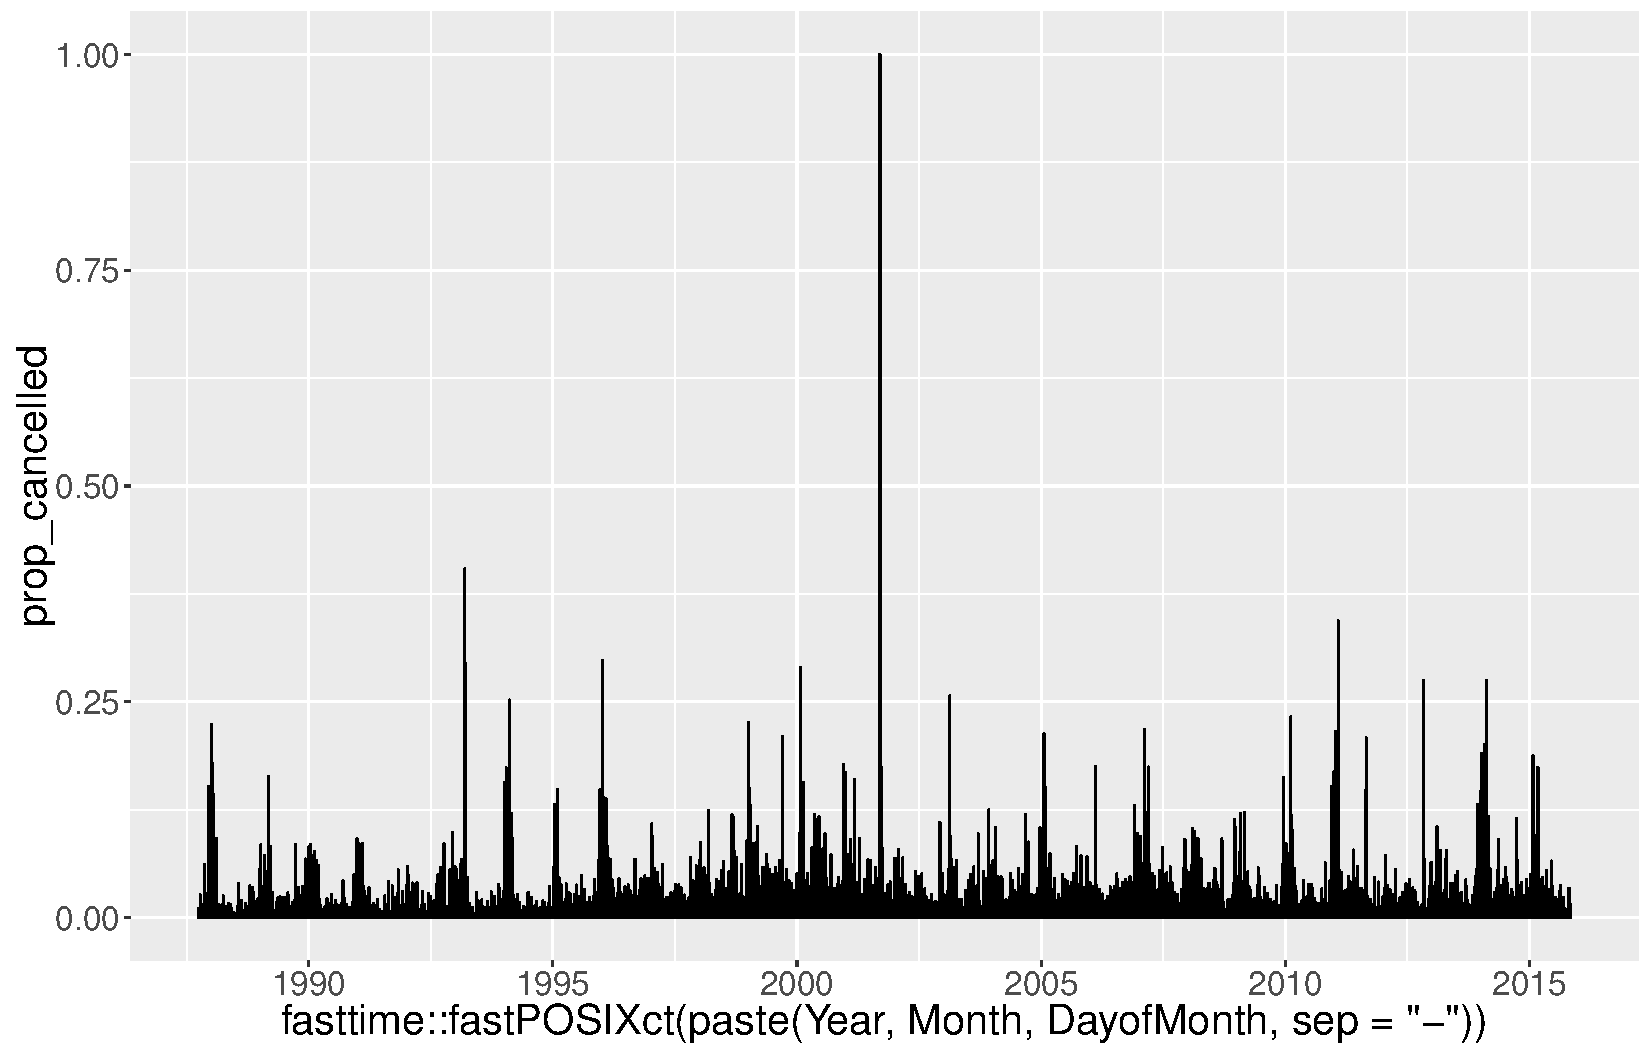
\includegraphics[width = \figurewidth]{figure/Cancellations-by-date-1}}
\caption{Proportion of flights cancelled by date.}
\end{figure}

\begin{knitrout}
\definecolor{shadecolor}{rgb}{0.969, 0.969, 0.969}\color{fgcolor}\begin{kframe}
\begin{alltt}
 \hlstd{flights} \hlopt
  \hlkwd{group_by}\hlstd{(Year, Month, DayofMonth)} \hlopt
  \hlkwd{summarise}\hlstd{(}\hlkwc{prop_cancelled} \hlstd{=} \hlkwd{mean}\hlstd{(Cancelled))} \hlopt
  \hlstd{ungroup} \hlopt
  \hlkwd{mutate}\hlstd{(}\hlkwc{rank} \hlstd{=} \hlkwd{dense_rank}\hlstd{(prop_cancelled))} \hlopt
  \hlkwd{ggplot}\hlstd{(}\hlkwd{aes}\hlstd{(}\hlkwc{x} \hlstd{=} \hlkwd{jitter}\hlstd{(rank,} \hlkwc{amount} \hlstd{=} \hlnum{0.1}\hlstd{),} \hlkwc{y} \hlstd{= prop_cancelled))} \hlopt{+} \hlkwd{geom_bar}\hlstd{(}\hlkwc{stat} \hlstd{=} \hlstr{"identity"}\hlstd{,} \hlkwc{width}\hlstd{=}\hlnum{1}\hlstd{)}
\end{alltt}


{\ttfamily\noindent\color{warningcolor}{\#\# Warning: position\_stack requires non-overlapping x intervals}}\end{kframe}
\end{knitrout}
\begin{figure}
{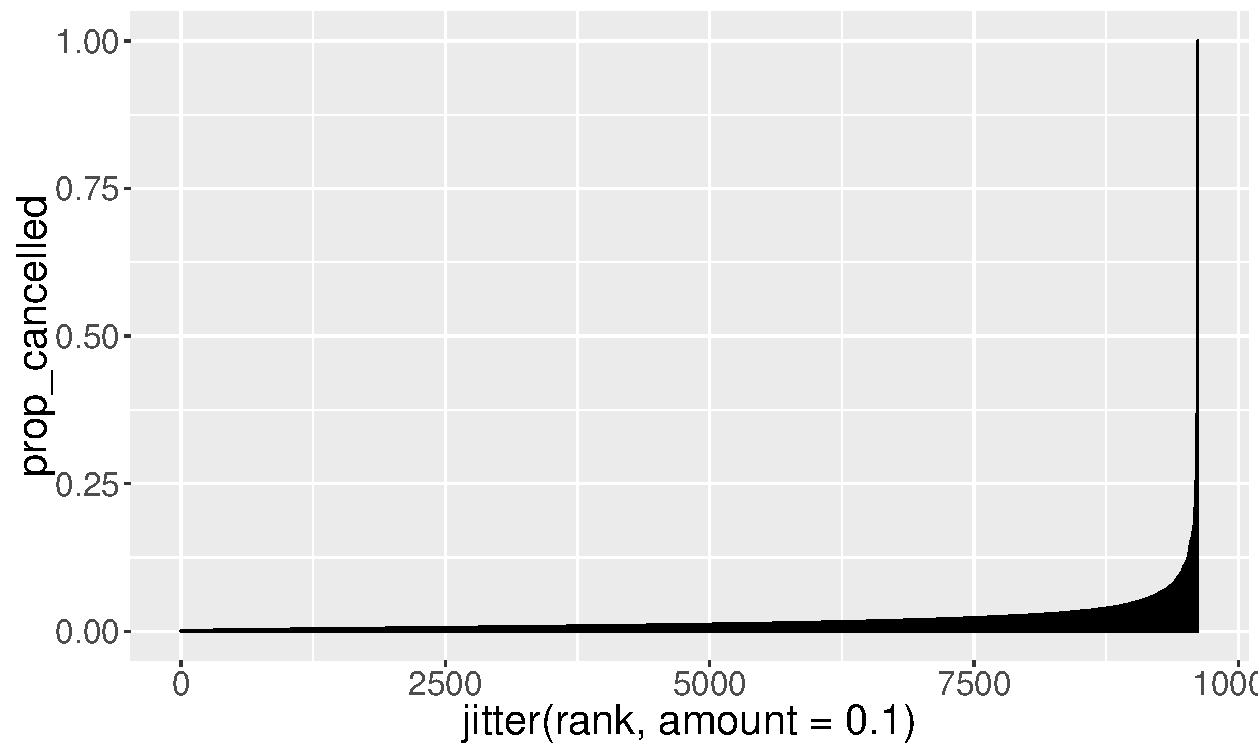
\includegraphics[width = \figurewidth]{figure/Sept11-cumulative-1}}
\caption{Pareto distribution of cancellation proportions.}
\end{figure}

\begin{knitrout}
\definecolor{shadecolor}{rgb}{0.969, 0.969, 0.969}\color{fgcolor}\begin{kframe}
\begin{alltt}
\hlstd{flights} \hlopt
  \hlkwd{filter}\hlstd{(Year} \hlopt{==} \hlnum{2001}\hlstd{, Month} \hlopt{==} \hlnum{9}\hlstd{, DayofMonth} \hlopt{==} \hlnum{11}\hlstd{)} \hlopt
  \hlkwd{group_by}\hlstd{(Origin)} \hlopt
  \hlkwd{summarise}\hlstd{(}\hlkwc{latest_departure} \hlstd{=} \hlkwd{max}\hlstd{(DepDateTimeZulu))} \hlopt
  \hlstd{ungroup} \hlopt
  \hlkwd{arrange}\hlstd{(latest_departure)} \hlopt
  \hlkwd{mutate}\hlstd{(}\hlkwc{number_airports_closed} \hlstd{=} \hlnum{1}\hlopt{:}\hlkwd{n}\hlstd{())} \hlopt
  \hlkwd{ggplot}\hlstd{(}\hlkwd{aes}\hlstd{(}\hlkwc{x} \hlstd{= latest_departure,} \hlkwc{y} \hlstd{= number_airports_closed))} \hlopt{+}
  \hlkwd{geom_line}\hlstd{(}\hlkwc{group} \hlstd{=} \hlnum{1}\hlstd{)} \hlopt{+}
  \hlkwd{geom_vline}\hlstd{(}\hlkwc{xintercept} \hlstd{=} \hlkwd{as.numeric}\hlstd{(}\hlkwd{as.POSIXct}\hlstd{(}\hlstr{"2001-09-11 09:17:00"}\hlstd{)))}
\end{alltt}
\end{kframe}
\end{knitrout}
\begin{figure}
\caption{Number of airports closed by UTC (determined by date of last departure)}
{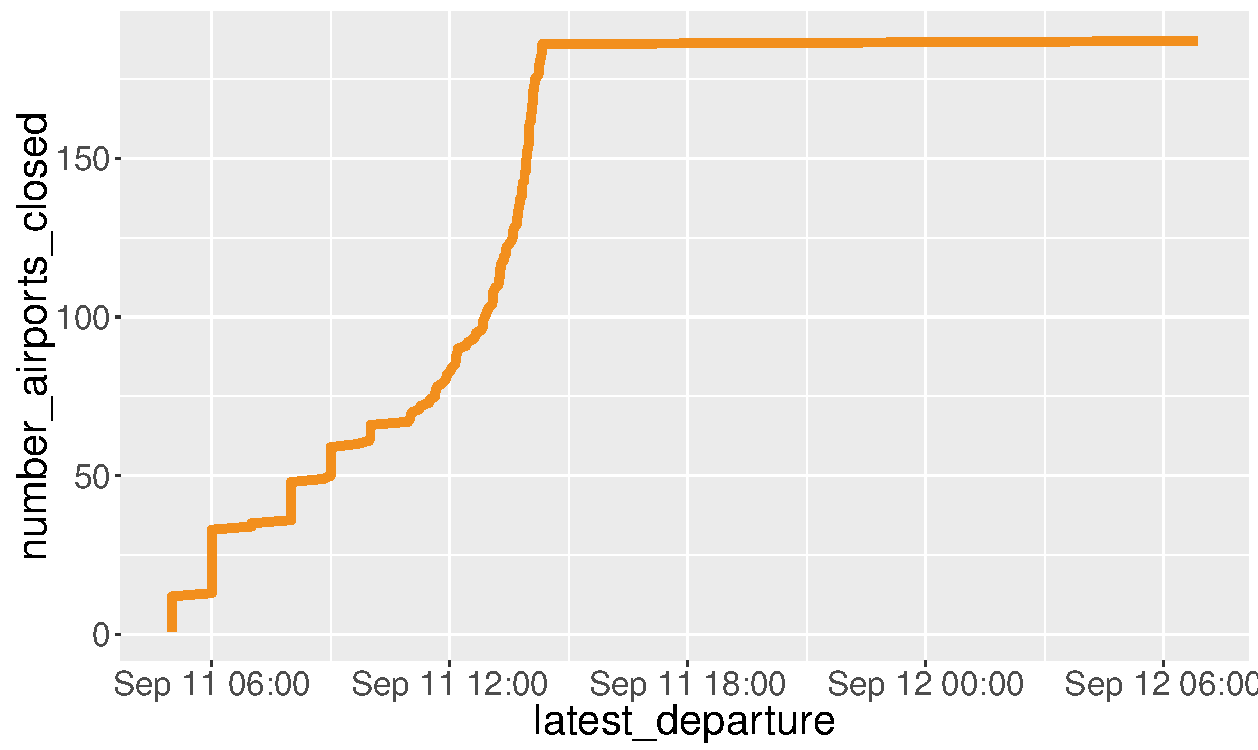
\includegraphics[width=\figurewidth]{figure/Sept11-airports-1}}
\end{figure}

\section{Atlanta, Chicago, and Dallas Fort-Worth}
\begin{knitrout}
\definecolor{shadecolor}{rgb}{0.969, 0.969, 0.969}\color{fgcolor}\begin{kframe}
\begin{alltt}
\hlstd{flights_hubs} \hlkwb{<-} \hlstd{flights[Origin} \hlopt \hlkwd{c}\hlstd{(}\hlstr{'ATL'}\hlstd{,} \hlstr{'ORD'}\hlstd{,} \hlstr{'DFW'}\hlstd{)]}
\end{alltt}
\end{kframe}
\end{knitrout}

\begin{knitrout}
\definecolor{shadecolor}{rgb}{0.969, 0.969, 0.969}\color{fgcolor}\begin{kframe}
\begin{alltt}
\hlstd{flights_hubs} \hlopt
  \hlkwd{filter}\hlstd{(Year} \hlopt{<} \hlnum{2015} \hlopt{|} \hlstd{Month} \hlopt{<} \hlnum{9}\hlstd{)} \hlopt
  \hlkwd{count}\hlstd{(Week, Origin)} \hlopt
  \hlkwd{setkey}\hlstd{(Week)} \hlopt
  \hlstd{data.table}\hlopt{:::}\hlkwd{merge.data.table}\hlstd{(}\hlkwd{unique}\hlstd{(unique_dates))} \hlopt
  \hlkwd{mutate}\hlstd{(}\hlkwc{Date} \hlstd{=} \hlkwd{as.Date}\hlstd{(}\hlkwd{paste0}\hlstd{(Year,} \hlstr{"-"}\hlstd{, Month,} \hlstr{"-"}\hlstd{, DayofMonth)))} \hlopt
  \hlkwd{ggplot}\hlstd{(}\hlkwd{aes}\hlstd{(}\hlkwc{x} \hlstd{= Date,} \hlkwc{y} \hlstd{= n} \hlopt{*} \hlstd{sample.weight.int,} \hlkwc{color} \hlstd{= Origin,} \hlkwc{group} \hlstd{= Origin))} \hlopt{+}
  \hlkwd{geom_line}\hlstd{()} \hlopt{+}
  \hlkwd{geom_point}\hlstd{()}
\end{alltt}
\end{kframe}
\end{knitrout}

\begin{knitrout}
\definecolor{shadecolor}{rgb}{0.969, 0.969, 0.969}\color{fgcolor}\begin{kframe}
\begin{alltt}
\hlstd{summary.tbl} \hlkwb{<-}
  \hlstd{flights_hubs} \hlopt
  \hlkwd{group_by}\hlstd{(Origin, Year, Month, DayofMonth)} \hlopt
  \hlkwd{summarise}\hlstd{(}\hlkwc{n} \hlstd{=} \hlkwd{n}\hlstd{(),} \hlkwc{average_delay} \hlstd{=} \hlkwd{sum}\hlstd{(DepDelay,} \hlkwc{na.rm} \hlstd{=} \hlnum{TRUE}\hlstd{)} \hlopt{/} \hlkwd{n}\hlstd{())}

\hlstd{average_delay_by_hub} \hlkwb{<-}
  \hlstd{summary.tbl} \hlopt
  \hlkwd{mutate}\hlstd{(}\hlkwc{Date} \hlstd{=} \hlkwd{as.Date}\hlstd{(}\hlkwd{paste0}\hlstd{(Year,} \hlstr{"-"}\hlstd{, Month, DayofMonth)))} \hlopt
  \hlkwd{ggplot}\hlstd{(}\hlkwd{aes}\hlstd{(}\hlkwc{x} \hlstd{= Date,} \hlkwc{y} \hlstd{= average_delay,} \hlkwc{group} \hlstd{= Origin,} \hlkwc{color} \hlstd{= Origin))} \hlopt{+}
  \hlkwd{geom_smooth}\hlstd{()}
\end{alltt}


{\ttfamily\noindent\bfseries\color{errorcolor}{\#\# Error in charToDate(x): character string is not in a standard unambiguous format}}\begin{alltt}
\hlstd{total_flights_by_hub} \hlkwb{<-}
  \hlstd{summary.tbl} \hlopt
  \hlkwd{mutate}\hlstd{(}\hlkwc{Date} \hlstd{=} \hlkwd{as.Date}\hlstd{(}\hlkwd{paste0}\hlstd{(Year,} \hlstr{"-"}\hlstd{, Month, DayofMonth)),}
         \hlkwc{n} \hlstd{= n} \hlopt{*} \hlstd{sample.weight.int)} \hlopt
  \hlkwd{ggplot}\hlstd{(}\hlkwd{aes}\hlstd{(}\hlkwc{x} \hlstd{= Date,} \hlkwc{y} \hlstd{= n))} \hlopt{+}
  \hlkwd{geom_smooth}\hlstd{(}\hlkwd{aes}\hlstd{(}\hlkwc{group} \hlstd{= Origin,} \hlkwc{color} \hlstd{= Origin))}
\end{alltt}


{\ttfamily\noindent\bfseries\color{errorcolor}{\#\# Error in charToDate(x): character string is not in a standard unambiguous format}}\begin{alltt}
\hlstd{gridExtra}\hlopt{::}\hlkwd{grid.arrange}\hlstd{(average_delay_by_hub, total_flights_by_hub,} \hlkwc{ncol} \hlstd{=} \hlnum{1}\hlstd{)}
\end{alltt}


{\ttfamily\noindent\bfseries\color{errorcolor}{\#\# Error in arrangeGrob(...): object 'average\_delay\_by\_hub' not found}}\end{kframe}
\end{knitrout}

\begin{knitrout}
\definecolor{shadecolor}{rgb}{0.969, 0.969, 0.969}\color{fgcolor}\begin{kframe}
\begin{alltt}
\hlstd{summary.tbl} \hlkwb{<-}
  \hlstd{flights_hubs} \hlopt
  \hlkwd{group_by}\hlstd{(Origin, Year, Month, DayofMonth)} \hlopt
  \hlkwd{summarise}\hlstd{(}\hlkwc{n} \hlstd{=} \hlkwd{n}\hlstd{(),} \hlkwc{total_depdelay} \hlstd{=} \hlkwd{sum}\hlstd{(DepDelay,} \hlkwc{na.rm} \hlstd{=} \hlnum{TRUE}\hlstd{)} \hlopt{/} \hlkwd{n}\hlstd{())}

\hlstd{summary.tbl} \hlopt \hlkwd{select}\hlstd{(}\hlopt{-}\hlstd{n)} \hlopt
  \hlstd{tidyr}\hlopt{::}\hlkwd{spread}\hlstd{(Origin, total_depdelay)} \hlopt
  \hlstd{tidyr}\hlopt{::}\hlkwd{gather}\hlstd{(Origin, dep_delay, DFW}\hlopt{:}\hlstd{ORD)} \hlopt
  \hlkwd{ggplot}\hlstd{(}\hlkwd{aes}\hlstd{(}\hlkwc{x} \hlstd{= ATL,} \hlkwc{y} \hlstd{= dep_delay,} \hlkwc{color} \hlstd{= Origin))} \hlopt{+}
  \hlkwd{geom_point}\hlstd{(}\hlkwc{alpha} \hlstd{=} \hlnum{0.051}\hlstd{)} \hlopt{+}
  \hlkwd{guides}\hlstd{(}\hlkwc{color} \hlstd{=} \hlkwd{guide_legend}\hlstd{(}\hlkwc{override.aes} \hlstd{=} \hlkwd{list}\hlstd{(}\hlkwc{size} \hlstd{=} \hlnum{4}\hlstd{)))} \hlopt{+}
  \hlkwd{theme}\hlstd{(}\hlkwc{legend.position} \hlstd{=} \hlkwd{c}\hlstd{(}\hlnum{0.8}\hlstd{,} \hlnum{0.8}\hlstd{))} \hlopt{+}
  \hlkwd{geom_smooth}\hlstd{()} \hlopt{+}
  \hlkwd{geom_abline}\hlstd{(}\hlkwc{slope} \hlstd{=} \hlnum{1}\hlstd{)} \hlopt{+}
  \hlkwd{coord_equal}\hlstd{()} \hlopt{+}
  \hlkwd{xlim}\hlstd{(}\hlopt{-}\hlnum{10}\hlstd{,}\hlnum{60}\hlstd{)} \hlopt{+} \hlkwd{ylim}\hlstd{(}\hlopt{-}\hlnum{10}\hlstd{,}\hlnum{60}\hlstd{)} \hlopt{+}
  \hlkwd{facet_grid}\hlstd{(Origin} \hlopt{~} \hlstd{.)}
\end{alltt}


{\ttfamily\noindent\color{warningcolor}{\#\# Warning: Removed 226 rows containing non-finite values (stat\_smooth).}}

{\ttfamily\noindent\color{warningcolor}{\#\# Warning: Removed 226 rows containing missing values (geom\_point).}}\end{kframe}
\end{knitrout}



\begin{knitrout}
\definecolor{shadecolor}{rgb}{0.969, 0.969, 0.969}\color{fgcolor}\begin{kframe}
\begin{alltt}
\hlstd{FINISH.TIME} \hlkwb{<-} \hlkwd{Sys.time}\hlstd{()}
\end{alltt}
\end{kframe}
\end{knitrout}
Compiled in 19.5275007327398
\end{document}
